\section{Разложение в ряд Фурье}

В общем случае частичная сумма ряда Фурье выглядит следующим образом: 
\begin{equation}
    F_N(t) = \frac{a_0}{2} + \sum\limits_{n=1}^{N} \left( a_n \cos(\omega_n t) + b_n \sin(\omega_n t) \right)
    \label{eq:fourier}
\end{equation}
\begin{equation}
    a_n = \frac{2}{T} \int\limits_{h}^{h + T} f(t) \cos(\omega_n t) dt ~~~~ b_n = \frac{2}{T} \int\limits_{h}^{h + T} f(t) \sin(\omega_n t) dt 
    \label{eq:fourier_coefficients}
\end{equation}
где $\omega_n = 2\pi n / T$, $h$ -- начало промежутка, на котором проводится разложение, $T$ -- период функции.

Или, для комплексного случая:
\begin{equation}
    G_N(t) = \sum\limits_{n = -N}^{N} c_n e^{i \omega_n t}
    \label{eq:fourier_exp}
\end{equation}
\begin{equation}
    c_n = \frac{1}{T}\int\limits_{h}^{h+T} f(t) e^{-i \omega_i t} dt 
    \label{eq:fourier_coefficients_exp}
\end{equation}
где $\omega_n = 2\pi n / T$,  $h$ -- начало промежутка, на котором проводится разложение, $T$ -- период функции.


\section{Вещественные функции}

\subsection{Квадратная волна}

Рассмотрим периодическую функцию с периодом $T = 3$:
\begin{equation}
    f_1(t) = 
    \begin{cases}
        1, & t \in [1, 2) \\
        2, & t \in [2, 4)
    \end{cases}
    \label{eq:func_1}
\end{equation}

График этой функции приведен на рис.~\ref{fig:func_1}. 
\begin{figure}[ht!]
    \centering
    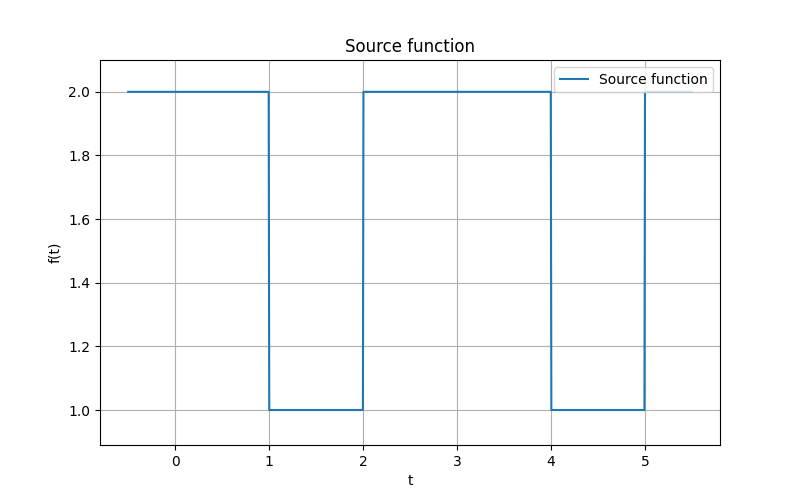
\includegraphics[width=\textwidth]{media/plots/func_1.png}
    \caption{График функции $f_1(t)$}
    \label{fig:func_1}
\end{figure}

\subsubsection{Вычисление коэффициентов Фурье}
Найдем частичные суммы ряда Фурье для этой функции:

Вычислим коэффициенты $a_n$, $b_n$ и $c_n$ для $n = 0, 1, 2$ в соответствии с формулами (\ref{eq:fourier_coefficients}) и (\ref{eq:fourier_coefficients_exp}): 

\begin{equation}
    a_n = \frac{2}{3} \int\limits_{1}^{4} f_1(t) \cos\left( \frac{2\pi n}{3} t\right) dt = \frac{2}{3} \left( \int\limits_{1}^{2} \cos\left( \frac{2\pi n}{3} t\right) dt + \int\limits_{2}^{4} 2 \cos\left( \frac{2\pi n}{3} t\right) dt \right) 
\end{equation}
\begin{equation}
    \int \cos\left( \frac{2\pi n}{3} t \right) dt = \int \frac{3\cos(u)}{2\pi n}du = \frac{3}{2\pi n } \sin(u) = \frac{3}{2\pi n } \sin\left( \frac{2\pi n}{3} t \right)
    \notag
 \end{equation}
\begin{multline}
    a_n = \frac{2}{3} \left( \frac{3}{2\pi n } \sin\left( \frac{2\pi n}{3} t \right) \Big|_{1}^{2}  + \frac{3}{\pi n } \sin\left( \frac{2\pi n}{3} t \right) \Big|_2^4 \right) = \\ 
    \frac{2}{\pi n} \left( \frac{1}{2} \left( \sin\left(\frac{4\pi n}{3}\right) - \sin\left(\frac{2\pi n}{3}\right) \right) + \left(\sin\left(\frac{8\pi n}{3}\right)  - \sin\left(\frac{4\pi n}{3}\right)  \right) \right) = \\
    \frac{1}{\pi n}\left(-\sin\left( \frac{4\pi n}{3}\right) - \sin\left(\frac{2\pi n}{3} \right) + 2\sin\left(\frac{8\pi n}{3}\right)\right)
\end{multline}
\begin{equation}
    b_n = \frac{2}{3} \int\limits_{1}^{4} f_1(t) \sin\left( \frac{2\pi n}{3} t\right) dt = \frac{2}{3} \left( \int\limits_{1}^{2} \sin\left( \frac{2\pi n}{3} t\right) dt + \int\limits_{2}^{4} 2 \sin\left( \frac{2\pi n}{3} t\right) dt \right) 
\end{equation}
\begin{equation}
    \int \sin\left( \frac{2\pi n}{3} t \right) dt = \int \frac{3\sin(u)}{2\pi n}du = \frac{-3}{2\pi n } \cos(u) = \frac{-3}{2\pi n } \cos\left( \frac{2\pi n}{3} t \right)
    \notag
 \end{equation}
\begin{multline}
    b_n = \frac{2}{3} \left( \frac{-3}{2\pi n } \cos\left( \frac{2\pi n}{3} t \right) \Big|_{1}^{2}  + \frac{-3}{\pi n } \cos\left( \frac{2\pi n}{3} t \right) \Big|_2^4 \right) = \\ 
    \frac{-2}{\pi n} \left( \frac{1}{2} \left( \cos\left(\frac{4\pi n}{3}\right) - \cos\left(\frac{2\pi n}{3}\right) \right) + \left(\cos\left(\frac{8\pi n}{3}\right)  - \cos\left(\frac{4\pi n}{3}\right)  \right) \right) = \\
    \frac{1}{\pi n}\left(\cos\left( \frac{4\pi n}{3}\right) + \cos\left(\frac{2\pi n}{3} \right) - 2\cos\left(\frac{8\pi n}{3}\right)\right)
\end{multline}
\begin{equation}
    c_n = \frac{1}{3}\int\limits_{1}^{4} f_1(t)e^{\frac{-i 2\pi n t}{3}} dt = \frac{1}{3}\left(\int\limits_{1}^{2}e^{\frac{-i 2\pi n t}{3}}dt + \int\limits_{2}^{4}2e^{\frac{-i 2\pi n t}{3}}dt \right) 
\end{equation}
Так как коэффициенты $a_n$, $b_n$ и $c_n$ связаны между собой, а $c_i$ и $c_{-i}$ равны для вещественной функции, нет необходимости вычислять $c_n$ отдельно. (Мне просто лень). 
\begin{equation}
    c_n = \frac{a_n - ib_n}{2}
\end{equation}
После подстановки получаем следующие значения:
\begin{equation}
    a_0 = \frac{2}{3} \int\limits_{1}^{4} f_1(t) dt = \frac{2}{3} \left( \int\limits_{1}^{2} dt + \int\limits_{2}^{4} 2 dt \right) = \frac{2}{3} \left(t\Big|_{1}^{2} + 2t\Big|_{2}^{4}\right) = \frac{2}{3} (1 + 4) = \frac{10}{3} \approx 3.33333
\end{equation}

\begin{equation}
    a_1 = \frac{1}{\pi}\left(-\sin\left( \frac{4\pi}{3}\right) - \sin\left(\frac{2\pi}{3} \right) + 2\sin\left(\frac{8\pi}{3}\right)\right) = \frac{\sqrt3}{3} \approx 0.55133 
\end{equation}

\begin{equation}
    a_2 = \frac{1}{2\pi}\left(-\sin\left( \frac{8\pi}{3}\right) - \sin\left(\frac{4\pi}{3} \right) + 2\sin\left(\frac{16\pi}{3}\right)\right) = \frac{-\sqrt{3}}{2\pi} \approx -0.27567
\end{equation}

\begin{equation}
    b_1 = \frac{1}{\pi}\left(\cos\left( \frac{4\pi}{3}\right) + \cos\left(\frac{2\pi}{3} \right) - 2\cos\left(\frac{8\pi}{3}\right)\right) = 0
\end{equation}

\begin{equation}
    b_2 = \frac{1}{2\pi}\left(\cos\left( \frac{8\pi}{3}\right) + \cos\left(\frac{4\pi}{3} \right) - 2\cos\left(\frac{16\pi}{3}\right)\right) = 0
\end{equation}

\begin{equation}
    c_0 = \frac{a_0}{2} = \frac{10}{6} \approx 1.66667
\end{equation}

\begin{equation}
    c_{-1} = c_1 = \frac{a_1 - b_1}{2} = \frac{\sqrt3}{6} \approx 0.28868
\end{equation}

\begin{equation}
    c_{-2} = c_2 = \frac{a_2 - b_2}{2} = \frac{-\sqrt{3}}{4\pi} \approx -0.13784
\end{equation}

\subsubsection{Вычисление коэффициентов Фурье с помощью программы}
Воспользуемся программой для вычисления коэффициентов Фурье. Исходный код всех функций приведен в дополнении \ref{appendix:source}.

\begin{lstlisting}[style=python_white, caption=Вычисление коэффициентов Фурье, label=lst:func_1]
func = np.vectorize(lambda x: 1 if 0 <= (x - 1) % 3 < 1 else 2)
a, b = fourier(func, 0, 2 * np.pi, 3)
print_fourier_coefficients(a, b)
c = fourier_exp(func, 1, 3, 3)
print_fourier_exp_coefficients(c)
\end{lstlisting}

В результате выполнения программы (\ref{lst:func_1}) получим следующие значения (см. таблицу~\ref{tab:func_1}~и~\ref{tab:func_1_exp}).

% table with coefficients
\begin{table}[ht!]
    \centering
    \begin{tabular}{|c|c|c|c|}
        \hline
        $n$ & $a_n$ & $b_n$ \\
        \hline
        0 & 3.33335 & 0.0 \\
        1 & 0.55123 & 0.0 \\
        2 & -0.2757 & 0.0 \\
        3 & 0.00020 & 0.0 \\
        \hline
    \end{tabular}
    \caption{Коэффициенты Фурье для функции $f_1(t)$}
    \label{tab:func_1}
\end{table}

\begin{table}[ht!]
    \centering
    \begin{tabular}{|c|c|}
        \hline
        $n$ & $c_n$ \\
        \hline
        -3 & 0.00010 \\
        -2 & -0.13788 \\
        -1 & 0.27561 \\
        0 & 1.66677 \\
        1 & 0.27561 \\
        2 & -0.13788 \\
        3 & 0.00010 \\
        \hline
    \end{tabular}
    \caption{Коэффициенты Фурье для функции $f_1(t)$ (комплексный случай)}
    \label{tab:func_1_exp}
\end{table}

Полученные коэффициенты совпадают с вычисленными вручную значениями.

\subsubsection{Построение графиков частичных сумм ряда Фурье}
В качество значений $N$ выберем $N = 1, 2, 5, 15, 30$. Для каждого значения $N$ вычислим частичную сумму ряда Фурье и построим график (см. рис.~\ref{fig:func_1_plot}~и~\ref{fig:func_1_plot_exp}).

\begin{lstlisting}[style=python_white, caption=Построение графиков частичных сумм ряда Фурье, label=lst:func_1_plot]
func = np.vectorize(lambda x: 1 if 0 <= (x - 1) % 3 < 1 else 2)
calc_and_plot(func, 1, 3, [1, 2, 5, 15, 30], './media/plots/func_1')
calc_and_plot_exp(func, 1, 3, [1, 2, 5, 15, 30], './media/plots/func_1_exp')
\end{lstlisting}

% plot with partial sums
\begin{figure}[ht!]
    \centering
    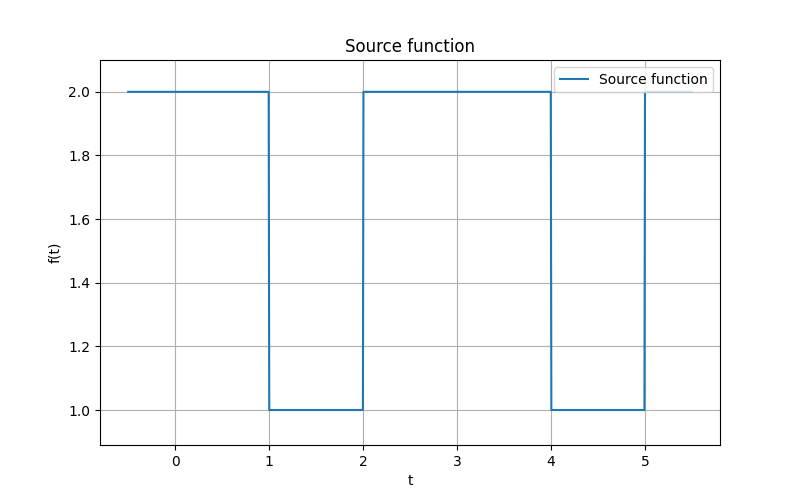
\includegraphics[width=0.49\textwidth]{media/plots/func_1.png}
    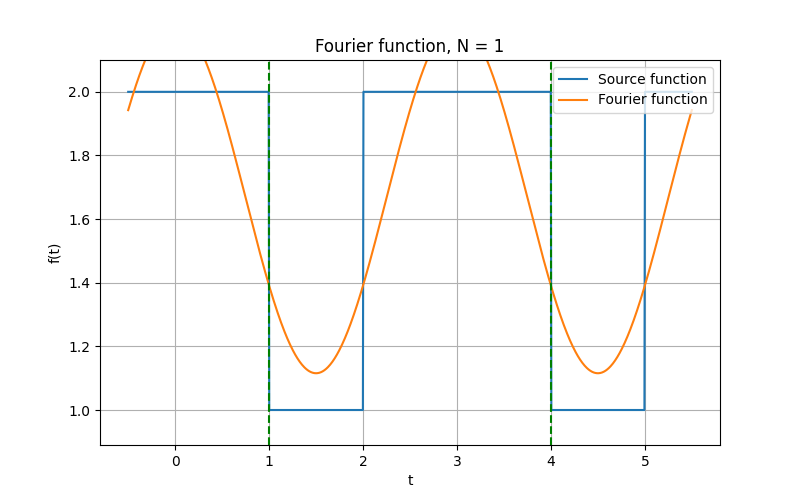
\includegraphics[width=0.49\textwidth]{media/plots/func_1_N_1.png}
    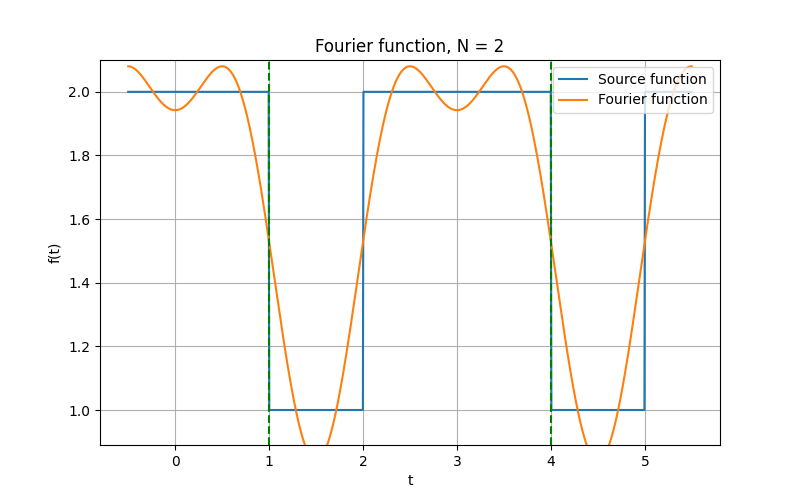
\includegraphics[width=0.49\textwidth]{media/plots/func_1_N_2.png}
    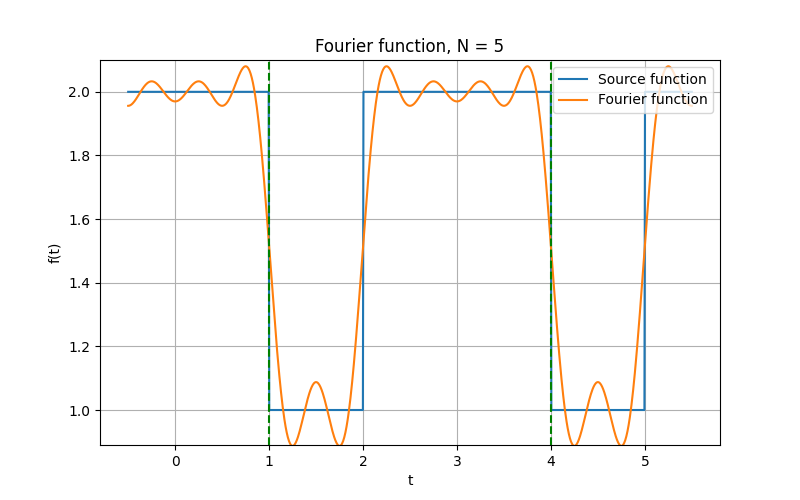
\includegraphics[width=0.49\textwidth]{media/plots/func_1_N_5.png}
    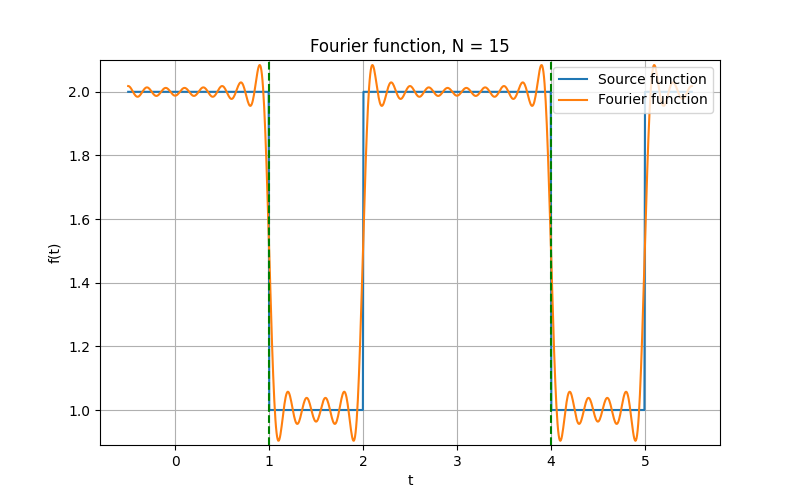
\includegraphics[width=0.49\textwidth]{media/plots/func_1_N_15.png}
    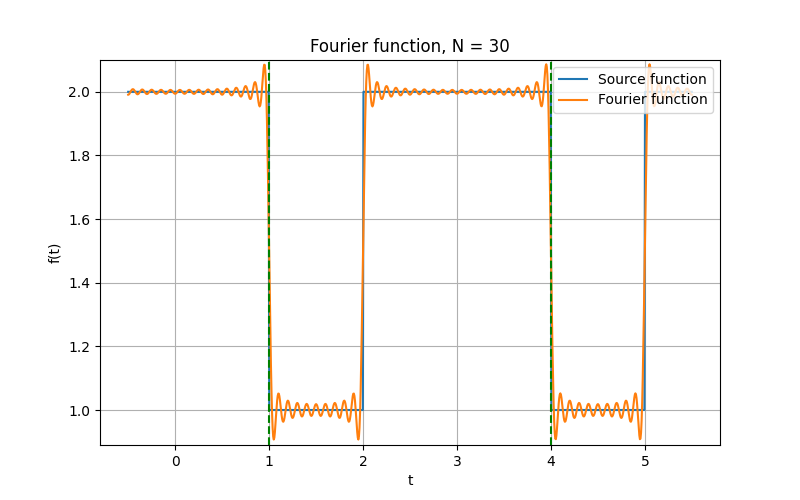
\includegraphics[width=0.49\textwidth]{media/plots/func_1_N_30.png}
    \caption{График частичных сумм ряда Фурье для функции $f_1(t)$}
    \label{fig:func_1_plot}
\end{figure}

\begin{figure}[ht!]
    \centering
    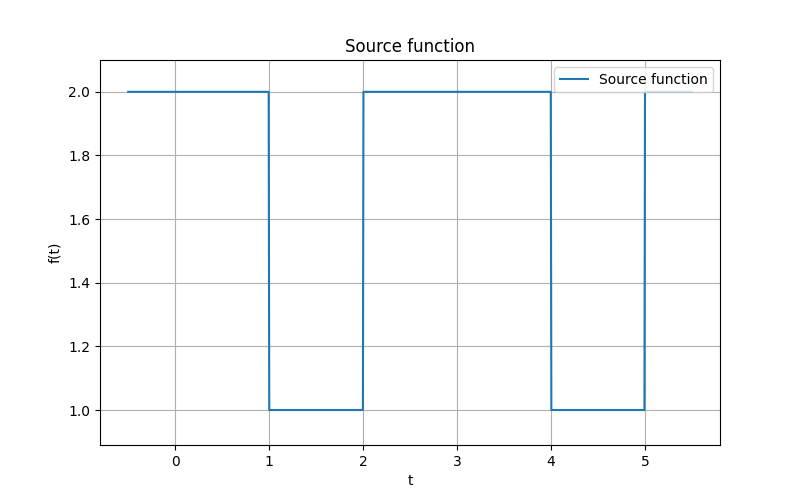
\includegraphics[width=0.49\textwidth]{media/plots/func_1_exp.png}
    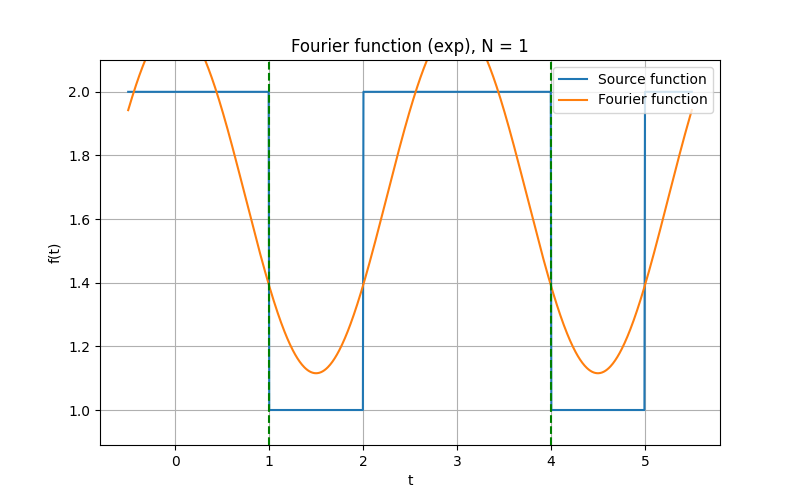
\includegraphics[width=0.49\textwidth]{media/plots/func_1_exp_N_1.png}
    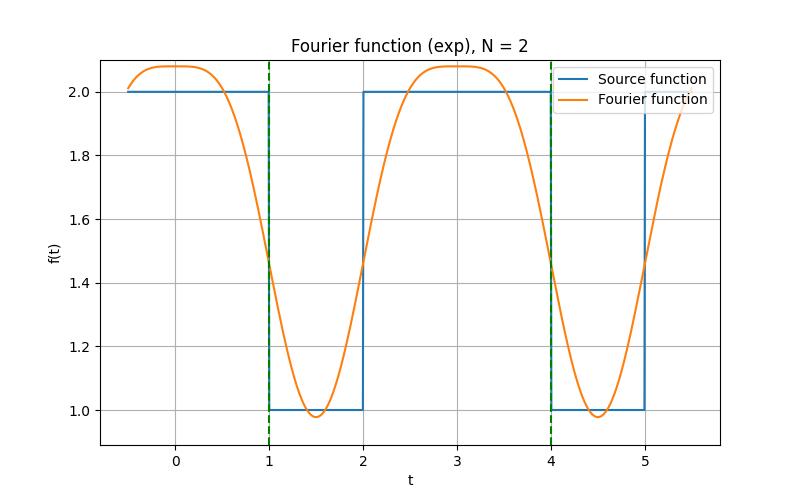
\includegraphics[width=0.49\textwidth]{media/plots/func_1_exp_N_2.png}
    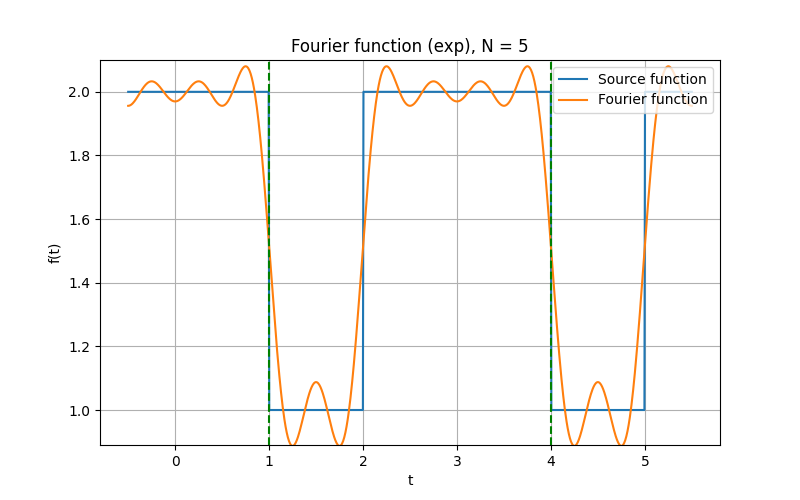
\includegraphics[width=0.49\textwidth]{media/plots/func_1_exp_N_5.png}
    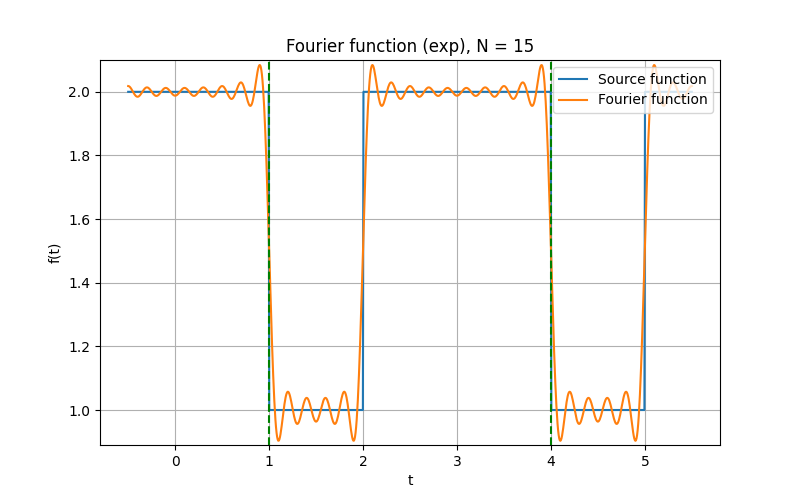
\includegraphics[width=0.49\textwidth]{media/plots/func_1_exp_N_15.png}
    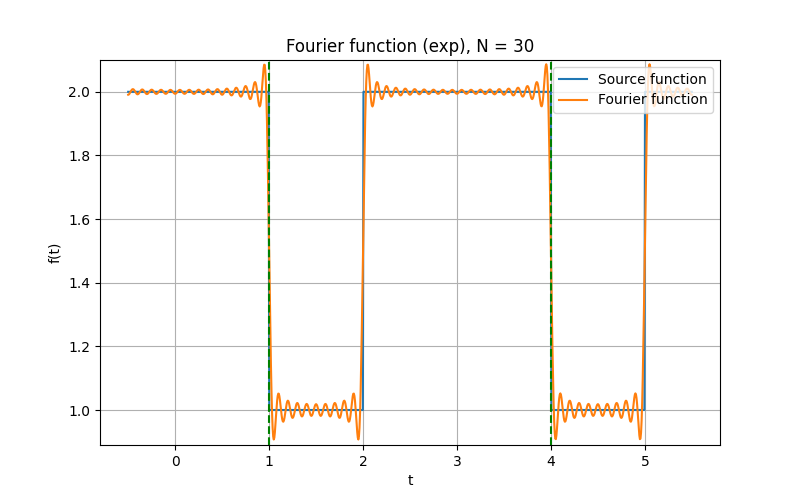
\includegraphics[width=0.49\textwidth]{media/plots/func_1_exp_N_30.png}
    \caption{График частичных сумм ряда Фурье для функции $f_1(t)$ (комплексный случай)}
    \label{fig:func_1_plot_exp}
\end{figure}

Видим, что при увеличении $N$ график частичной суммы ряда Фурье приближается к исходной функции. При $N = 5$ график частичной суммы ряда Фурье уже довольно хорошо приближает исходную функцию. 

На графиках заметны \textit{выбросы} в точках разрыва. Это связано с тем, что ряд Фурье сходится к функции по норме, но не обязательно в каждой точке. 

\FloatBarrier
\subsubsection{Проверка равенства Парсеваля}

Проверим равенство Парсеваля для функции $f_1(t)$:

\begin{equation}
    ||f_1||^2 = 2\pi \sum\limits_{n = -\infty}^{\infty} |c_n|^2 
\end{equation}

\begin{equation}
    ||f_1||^2 = \pi \left(\frac{a_0^2}{2} + \sum\limits_{n = 0}^{\infty}  (a_n^2 + b_n^2) \right)
\end{equation}

Для этого воспользуемся функцией \texttt{perseval\_check} (см. листинг~\ref{lst:perseval_check}).
Мною была рассмотрена сумма трехсот коэффициентов. Этого оказалось достаточно для равенства квадрата нормы и суммы до 3 знака. 

\begin{table}[ht!]
    \centering
    \begin{tabular}{|c|c|c|}
        \hline
        $||f_1||^2$ & $2\pi \sum\limits_{n = -\infty}^{300} |c_n|^2$ & $\pi \left(\frac{a_0^2}{2} + \sum\limits_{n = 1}^{300} (a_n^2 + b_n^2)\right)$\\
        \hline
        19.13296 & 19.13141 & 19.13141\\
        \hline
    \end{tabular}
    \caption{Проверка равенства Персеваля для функции $f_1(t)$}
    \label{tab:func_1_pers}
\end{table}
 
\FloatBarrier

\subsection{Четная функция}

Рассмотрим четную периодическую функцию с периодом $T = 2\pi$:

\begin{equation}
    f_2(t) = \sin\left(\frac{5}{2} \cos(t)\right)
\end{equation}

График этой функции приведен на рис.~\ref{fig:func_2}.

\begin{figure}[h!]
    \centering
    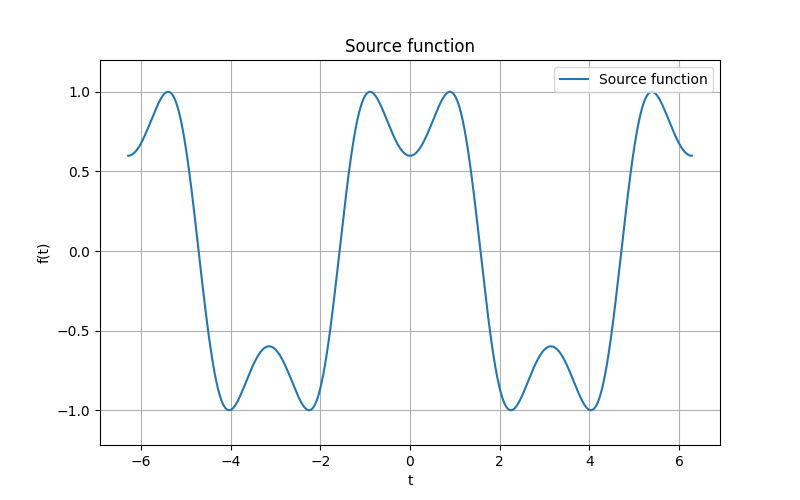
\includegraphics[width=\textwidth]{media/plots/func_2.png}
    \caption{График функции $f_2(t)$}
    \label{fig:func_2}
\end{figure}

\subsubsection{Вычисление коэффициентов Фурье}
Найдем коэффициенты ряда Фурье для этой функции:

\begin{equation}
    a_n = \frac{1}{\pi}\int\limits_{-\pi}^{\pi} \sin\left(\frac{5}{2} \cos\left(t\right)\right)\cos\left( n t \right) dt 
\end{equation}

\begin{equation}
    b_n = \frac{1}{\pi}\int\limits_{-\pi}^{\pi} \sin\left(\frac{5}{2} \cos\left(t\right)\right)\sin\left( n t \right) dt 
\end{equation}

\begin{equation}
    c_n = \frac{1}{2\pi}\int\limits_{-\pi}^{\pi}  \sin\left(\frac{5}{2} \cos\left(t\right)\right) e^{-int} dt 
\end{equation}

Уууупс, неберущийся интеграл... Ну а кому его брать то надо? Мне не надо, я поплакался в чате :)

\subsubsection{Вычисление коэффициентов Фурье с помощью программы}

\begin{lstlisting}[style=python_white, caption=Вычисление коэффициентов Фурье, label=lst:func_2]
func = np.vectorize(lambda x: np.sin(5/2 * np.cos(x)))
a, b = fourier(func, -np.pi, 2*np.pi, 3)
print_fourier_coefficients(a, b)
c = fourier_exp(func, -np.pi, 2*np.pi, 3)
print_fourier_exp_coefficients(c)
\end{lstlisting}

В результате выполнения программы (\ref{lst:func_2}) получим следующие значения (см. таблицу~\ref{tab:func_2}~и~\ref{tab:func_2_exp})~.

% table with coefficients
\begin{table}[h!]
    \centering
    \begin{tabular}{|c|c|c|}
        \hline
        $n$ & $a_n$ & $b_n$ \\
        \hline
        0 & 0.00012 & 0.0\\
        1 & 0.99431 & 0.0\\
        2 & 0.00012 & 0.0\\
        3 & -0.43308 & 0.0\\
        \hline
    \end{tabular}
    \caption{Коэффициенты Фурье для функции $f_2(t)$}
    \label{tab:func_2}
\end{table}

\begin{table}[h!]
    \centering
    \begin{tabular}{|c|c|}
        \hline
        $n$ & $c_n$ \\
        \hline
        -3 & -0.21654 \\
        -2 & -0.00006 \\
        -1 & 0.49715 \\
        0 & 0.00006 \\
        1 & 0.49715 \\
        2 & 0.00006 \\
        3 & -0.21654 \\
        \hline
    \end{tabular}
    \caption{Коэффициенты Фурье для функции $f_2(t)$ (комплексный случай)}
    \label{tab:func_2_exp}
\end{table}

\subsubsection{Построение графиков частичных сумм ряда Фурье}
В качество значений $N$ выберем $N = 1, 2, 3, 4, 5$. Для каждого значения $N$ вычислим частичную сумму ряда Фурье и построим график (см. рис.~\ref{fig:func_2_plot}~и~\ref{fig:func_2_plot_exp}).

\begin{lstlisting}[style=python_white, caption=Построение графиков частичных сумм ряда Фурье, label=lst:func_1_plot]
func = np.vectorize(lambda x: np.sin(5/2 * np.cos(x)))
calc_and_plot(func, -np.pi, 2 * np.pi, [1, 2, 3, 4, 5], './media/plots/func_2')
calc_and_plot_exp(func, -np.pi, 2 * np.pi, [1, 2, 3, 4, 5], './media/plots/func_2_exp')
\end{lstlisting}

% plot with partial sums
\begin{figure}[ht!]
    \centering
    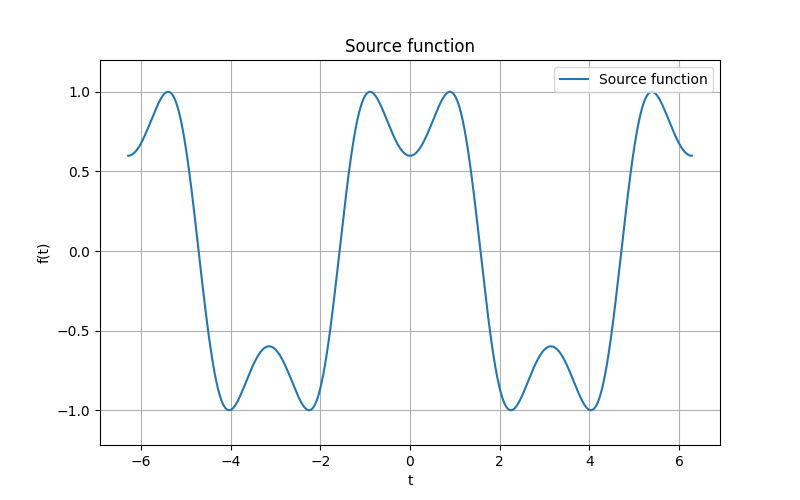
\includegraphics[width=0.49\textwidth]{media/plots/func_2.png}
    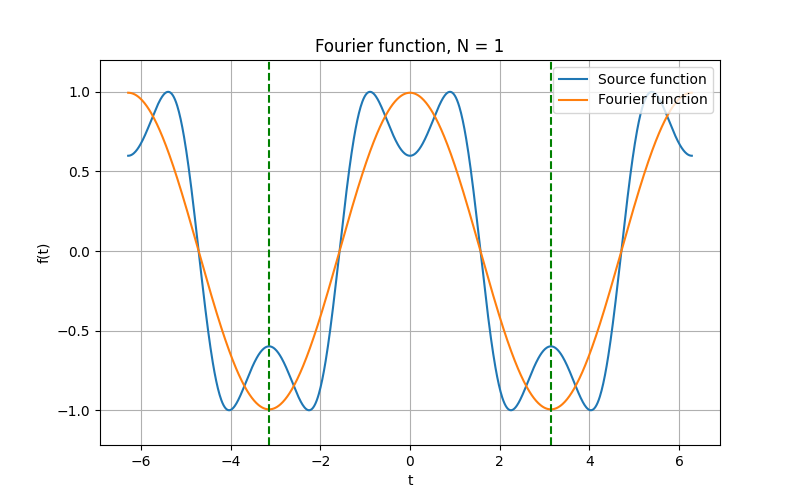
\includegraphics[width=0.49\textwidth]{media/plots/func_2_N_1.png}
    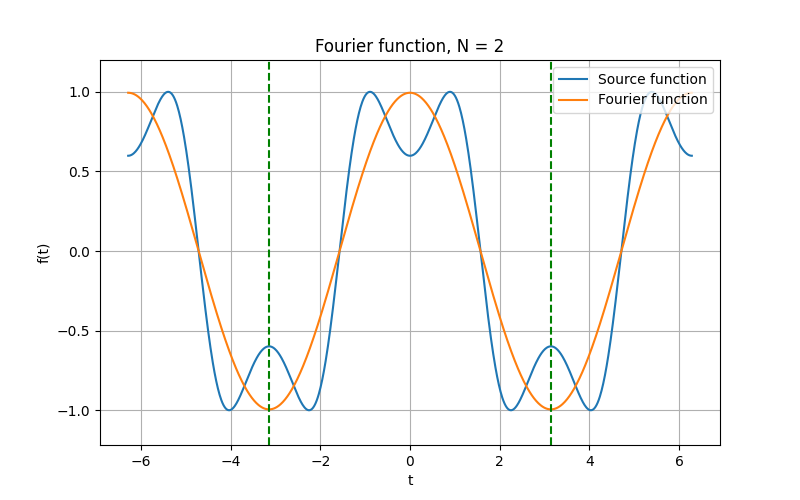
\includegraphics[width=0.49\textwidth]{media/plots/func_2_N_2.png}
    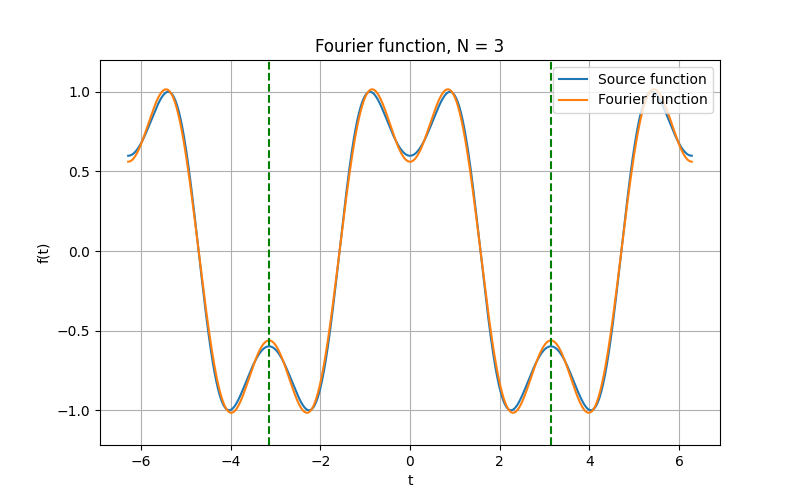
\includegraphics[width=0.49\textwidth]{media/plots/func_2_N_3.png}
    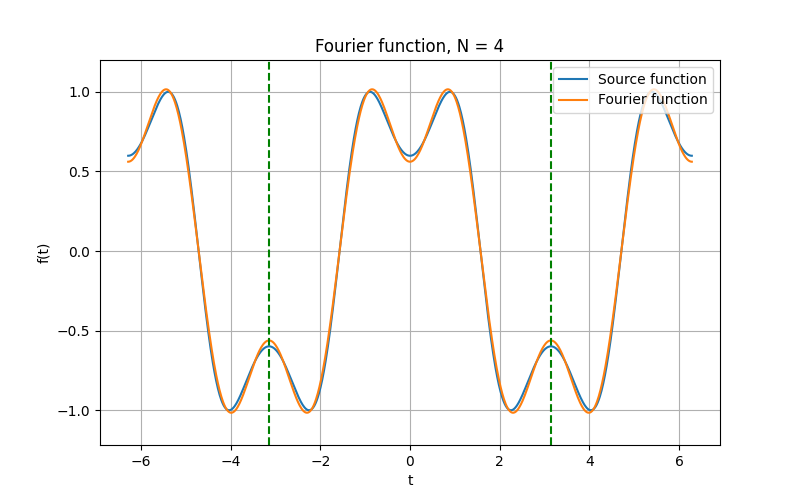
\includegraphics[width=0.49\textwidth]{media/plots/func_2_N_4.png}
    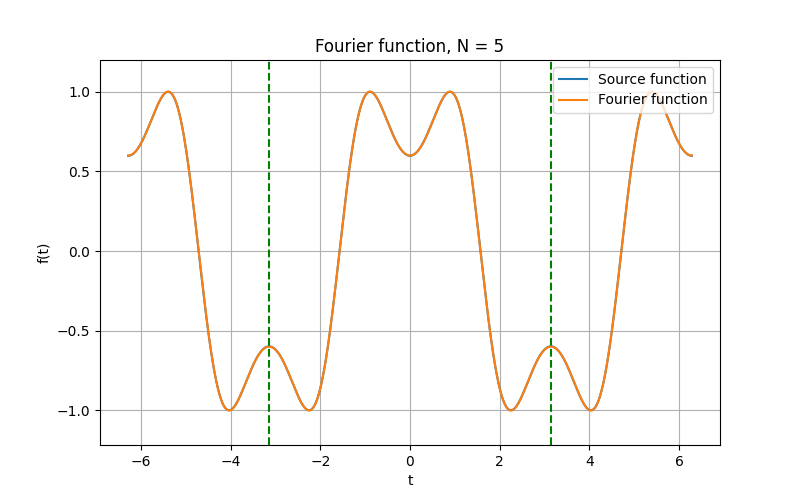
\includegraphics[width=0.49\textwidth]{media/plots/func_2_N_5.png}
    \caption{График частичных сумм ряда Фурье для функции $f_2(t)$}
    \label{fig:func_2_plot}
\end{figure}

\begin{figure}[ht!]
    \centering
    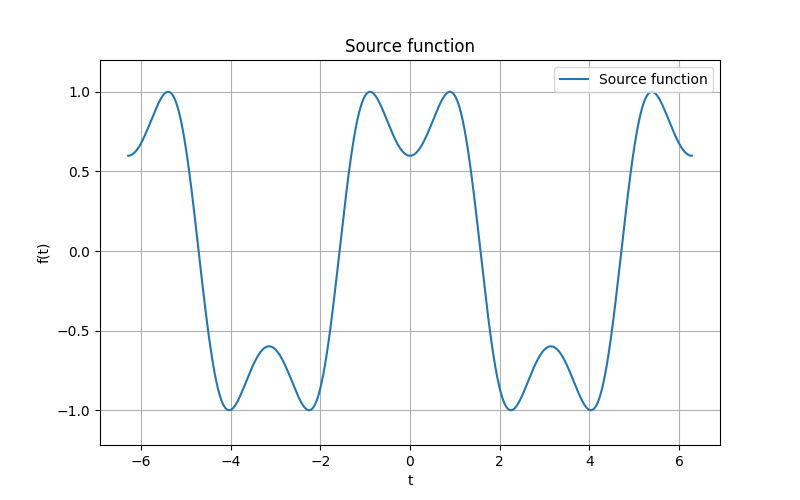
\includegraphics[width=0.49\textwidth]{media/plots/func_2_exp.png}
    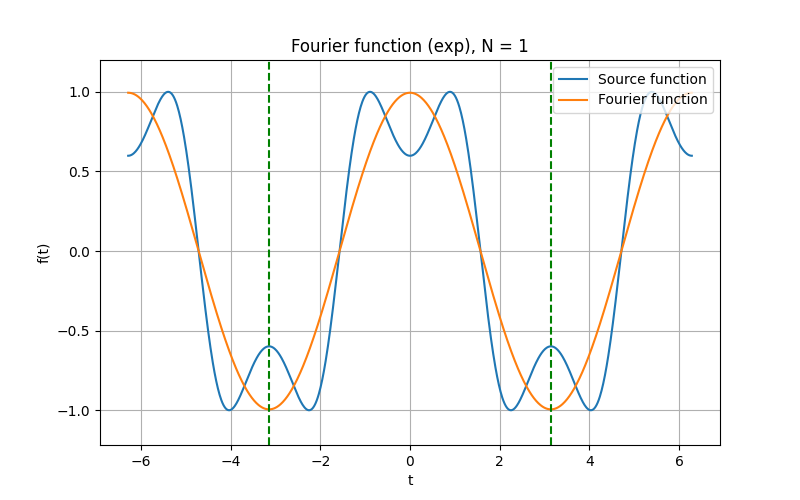
\includegraphics[width=0.49\textwidth]{media/plots/func_2_exp_N_1.png}
    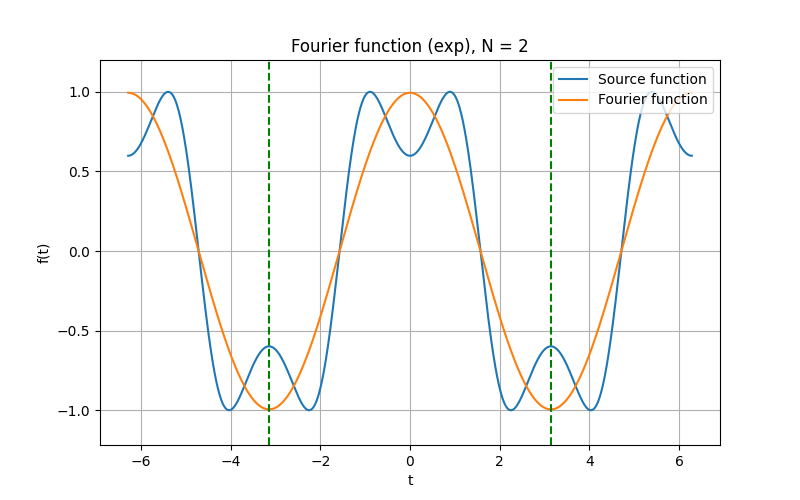
\includegraphics[width=0.49\textwidth]{media/plots/func_2_exp_N_2.png}
    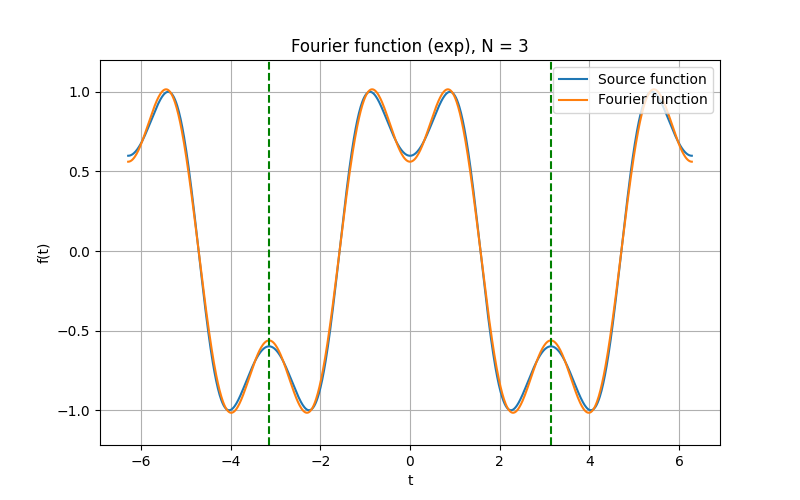
\includegraphics[width=0.49\textwidth]{media/plots/func_2_exp_N_3.png}
    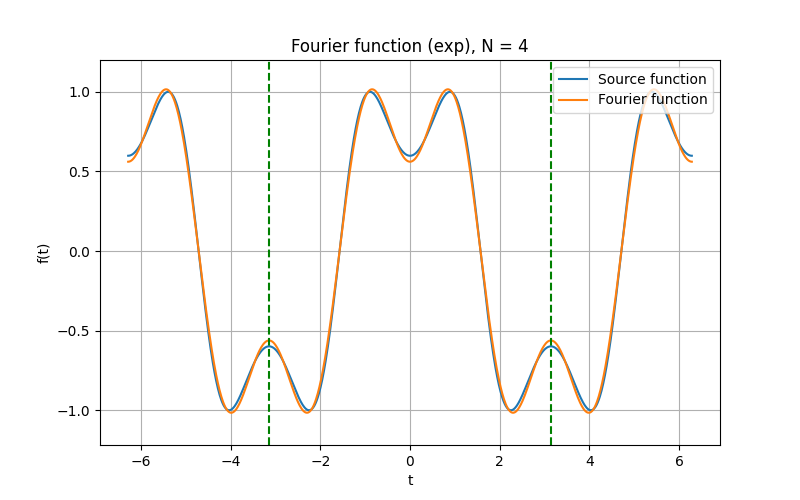
\includegraphics[width=0.49\textwidth]{media/plots/func_2_exp_N_4.png}
    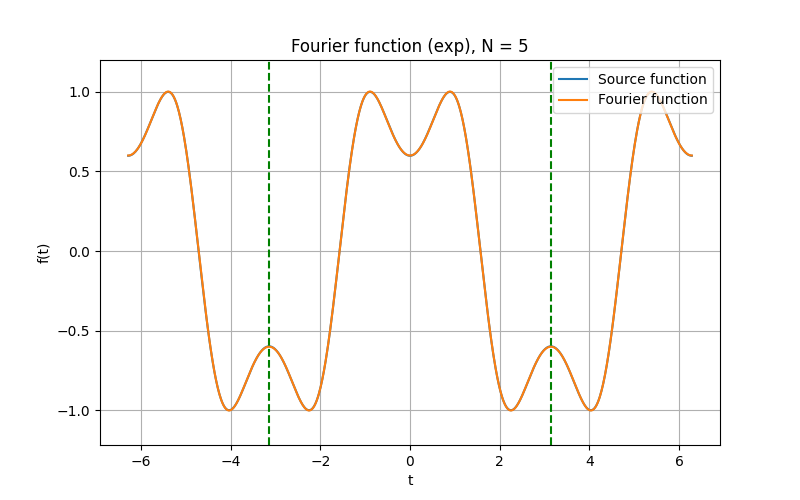
\includegraphics[width=0.49\textwidth]{media/plots/func_2_exp_N_5.png}
    \caption{График частичных сумм ряда Фурье для функции $f_2(t)$ (комплексный случай)}
    \label{fig:func_2_plot_exp}
\end{figure}

Видим, что при увеличении $N$ график частичной суммы ряда Фурье приближается к исходной функции. При $N = 5$ график частичной суммы ряда Фурье уже неотличим от исходной функции.
 
\FloatBarrier

\subsection{Нечетная функция}

Рассмотрим нечетную периодическую функцию с периодом $T = \pi$:

\begin{equation}
    f_3(t) = |\cos(2t) \cdot \sin(t)|
\end{equation}

График этой функции приведен на рис.~\ref{fig:func_3}.

\begin{figure}[ht!]
    \centering
    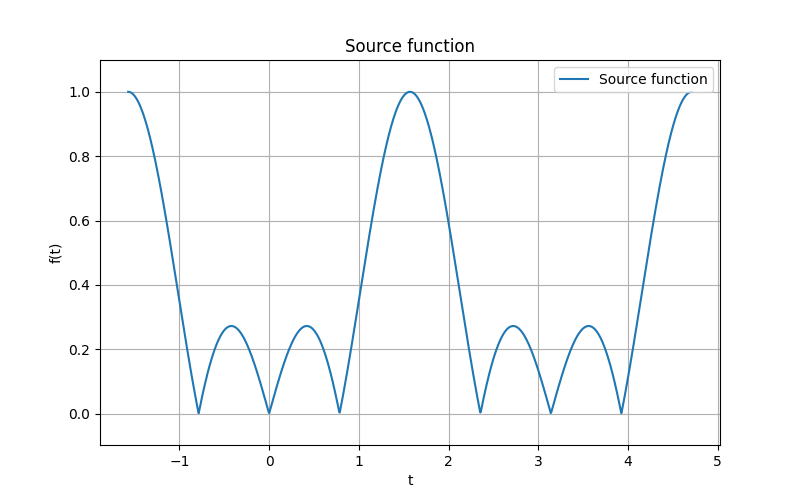
\includegraphics[width=\textwidth]{media/plots/func_3.png}
    \caption{График функции $f_3(t)$}
    \label{fig:func_3}
\end{figure}

\subsubsection{Вычисление коэффициентов Фурье}
Найдем коэффициенты ряда Фурье для этой функции:

\begin{equation}
    a_n = \frac{2}{\pi}\int\limits_{0}^{\pi} |\cos(2t) \cdot \sin(t)| \cos(2nt) dt 
\end{equation}

\begin{equation}
    b_n = \frac{2}{\pi}\int\limits_{0}^{\pi} |\cos(2t) \cdot \sin(t)| \sin(2nt) dt 
\end{equation}

\begin{equation}
    c_n = \frac{1}{\pi}\int\limits_{0}^{\pi} |\cos(2t) \cdot \sin(t)| e^{-2int} dt 
\end{equation}


\subsubsection{Вычисление коэффициентов Фурье с помощью программы}

\begin{lstlisting}[style=python_white, caption=Вычисление коэффициентов Фурье, label=lst:func_3]
func = np.vectorize(lambda x: abs(np.cos(2 * x) * np.sin(x)))
a, b = fourier(func, 0, np.pi, 3)
print_fourier_coefficients(a, b)
c = fourier_exp(func, 0, np.pi, 3)
print_fourier_exp_coefficients(c)
\end{lstlisting}

В результате выполнения программы (\ref{lst:func_3}) получим следующие значения (см. таблицу~\ref{tab:func_3}~и~\ref{tab:func_3_exp}).

% table with coefficients
\begin{table}[ht!]
    \centering
    \begin{tabular}{|c|c|c|}
        \hline
        $n$ & $a_n$ & $b_n$ \\
        \hline
        0 & 0.77601 & 0.0 \\
        1 & -0.36616 & 0.0 \\
        2 & 0.21548 & 0.0 \\
        3 & -0.09828 & 0.0 \\
        \hline
    \end{tabular}
    \caption{Коэффициенты Фурье для функции $f_3(t)$}
    \label{tab:func_3}
\end{table}

\begin{table}[ht!]
    \centering
    \begin{tabular}{|c|c|}
        \hline
        $n$ & $c_n$ \\
        \hline
        -3 & -0.04914 \\
        -2 & 0.10774 \\
        -1 & -0.18308 \\
        0 & 0.38800 \\
        1 & -0.18308 \\
        2 & 0.10774 \\
        3 & -0.04914 \\
        \hline
    \end{tabular}
    \caption{Коэффициенты Фурье для функции $f_3(t)$ (комплексный случай)}
    \label{tab:func_3_exp}
\end{table}

\subsubsection{Построение графиков частичных сумм ряда Фурье}
В качество значений $N$ выберем $N = 1, 2, 3, 4, 5$. Для каждого значения $N$ вычислим частичную сумму ряда Фурье и построим график (см. рис.~\ref{fig:func_3_plot}~и~\ref{fig:func_3_plot_exp}).

\begin{lstlisting}[style=python_white, caption=Построение графиков частичных сумм ряда Фурье, label=lst:func_1_plot]
func = np.vectorize(lambda x: abs(np.cos(2 * x) * np.sin(x)))
calc_and_plot(func, 0, np.pi, [1, 2, 3, 4, 5], './media/plots/func_3')
calc_and_plot_exp(func, 0, np.pi, [1, 2, 3, 4, 5], './media/plots/func_3_exp')
\end{lstlisting}

% plot with partial sums
\begin{figure}[ht!]
    \centering
    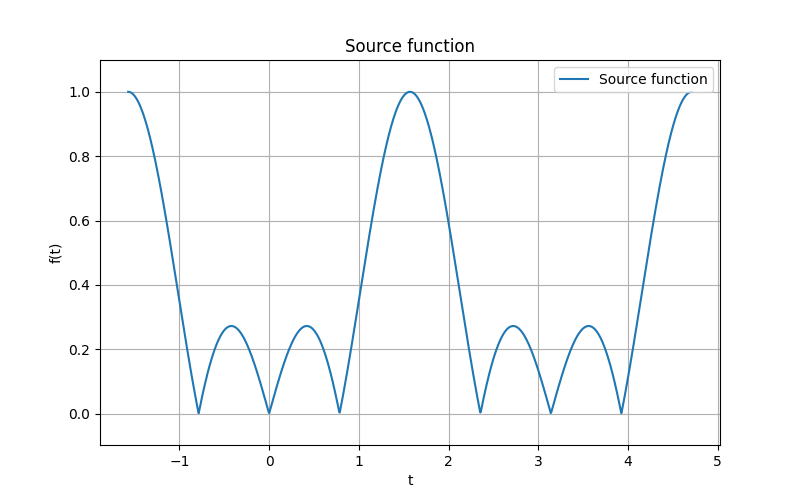
\includegraphics[width=0.49\textwidth]{media/plots/func_3_exp.png}
    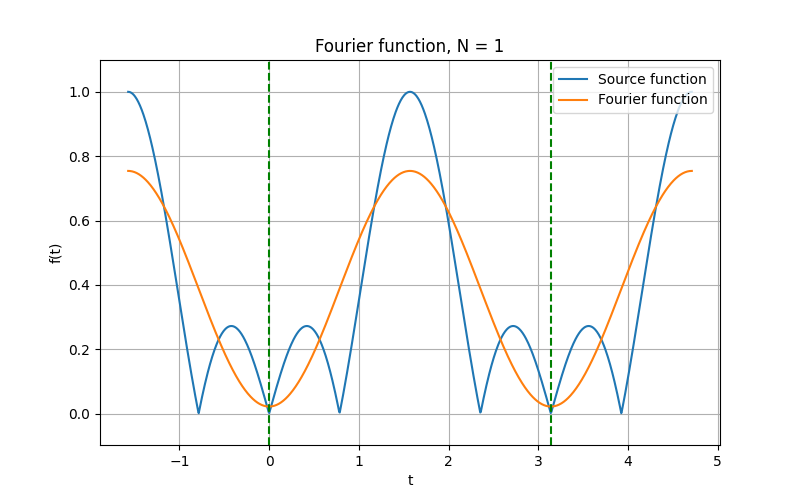
\includegraphics[width=0.49\textwidth]{media/plots/func_3_N_1.png}
    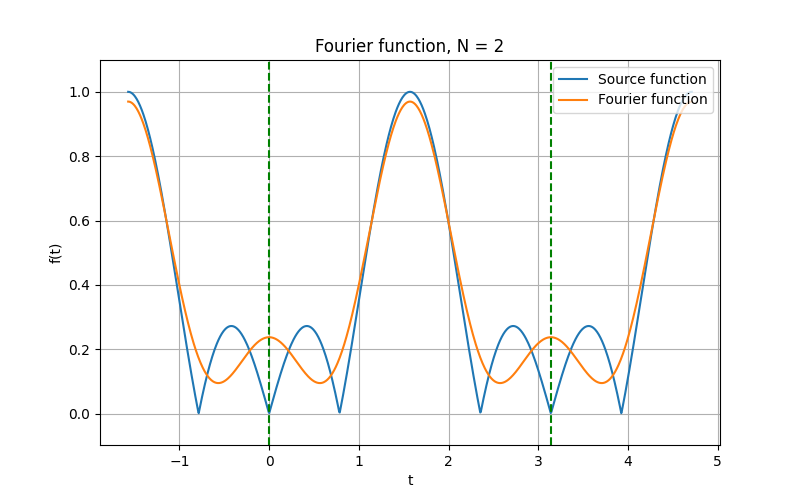
\includegraphics[width=0.49\textwidth]{media/plots/func_3_N_2.png}
    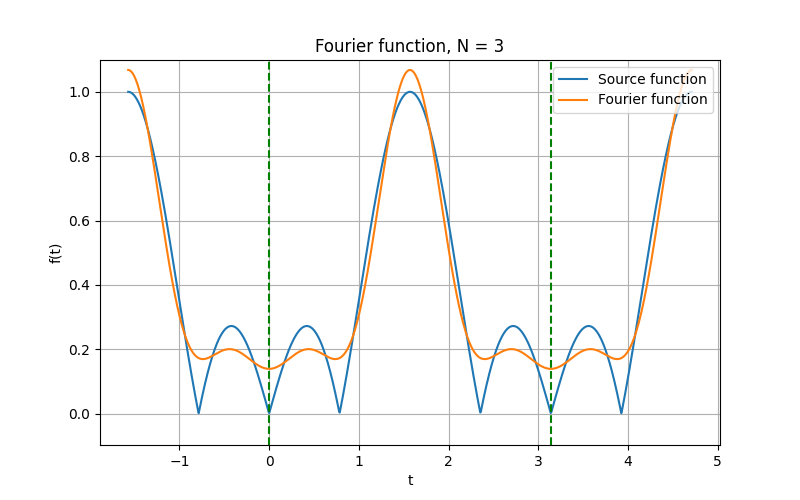
\includegraphics[width=0.49\textwidth]{media/plots/func_3_N_3.png}
    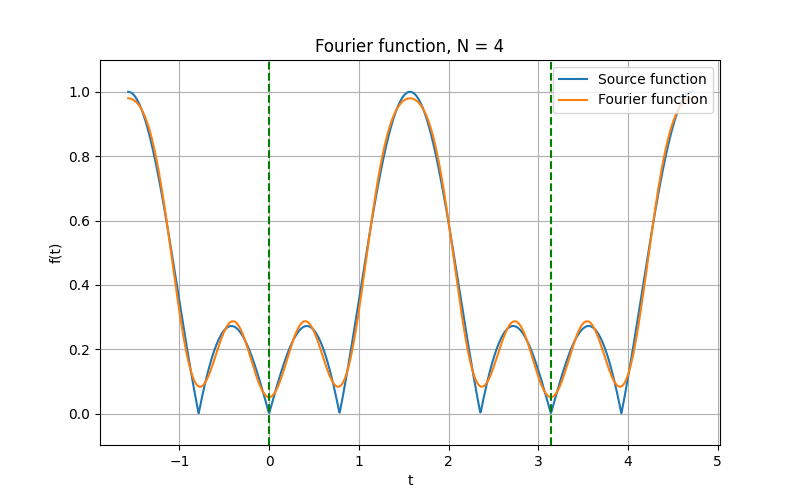
\includegraphics[width=0.49\textwidth]{media/plots/func_3_N_4.png}
    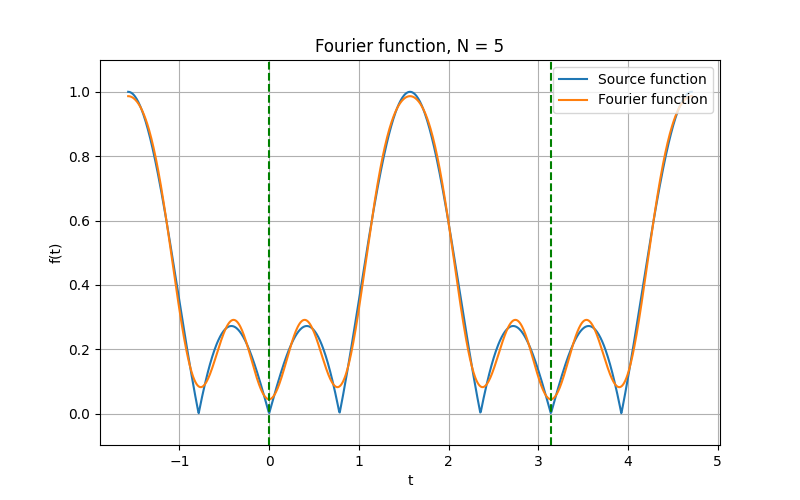
\includegraphics[width=0.49\textwidth]{media/plots/func_3_N_5.png}
    \caption{График частичных сумм ряда Фурье для функции $f_3(t)$}
    \label{fig:func_3_plot}
\end{figure}

\begin{figure}[ht!]
    \centering
    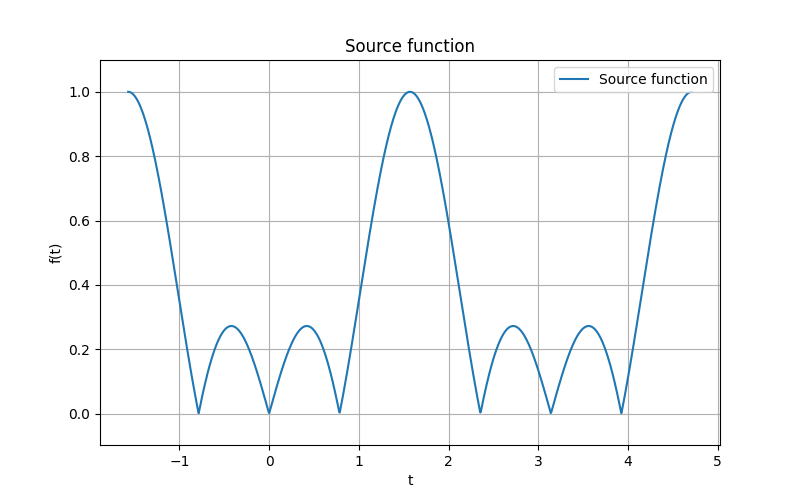
\includegraphics[width=0.49\textwidth]{media/plots/func_3.png}
    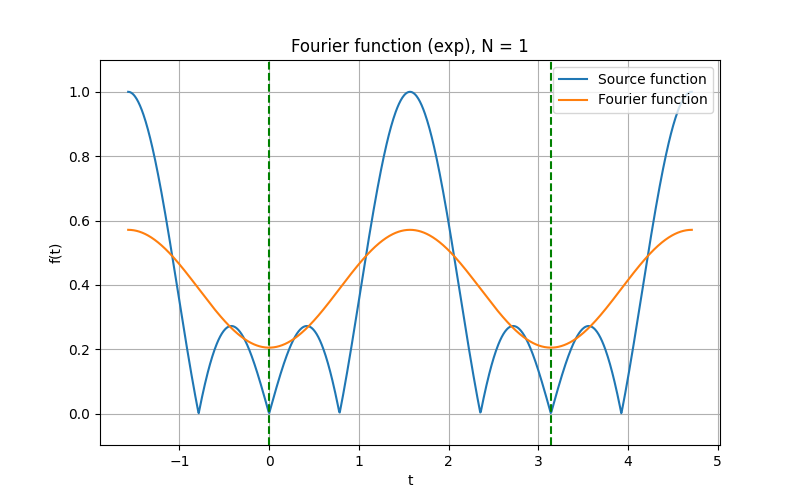
\includegraphics[width=0.49\textwidth]{media/plots/func_3_exp_N_1.png}
    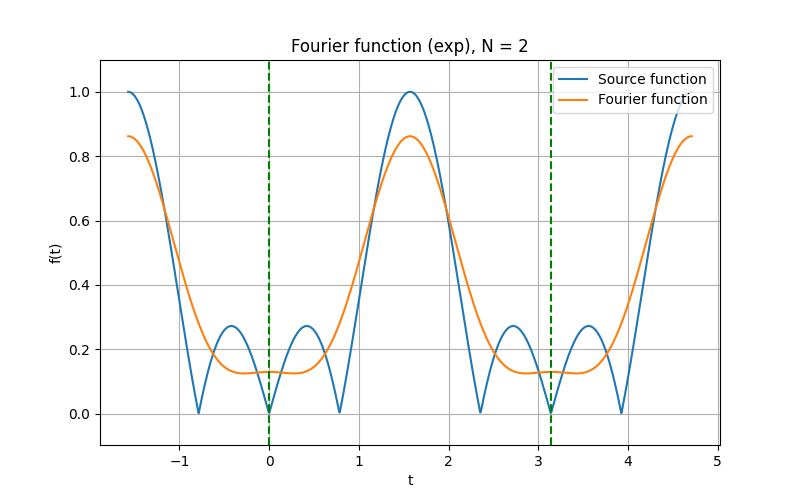
\includegraphics[width=0.49\textwidth]{media/plots/func_3_exp_N_2.png}
    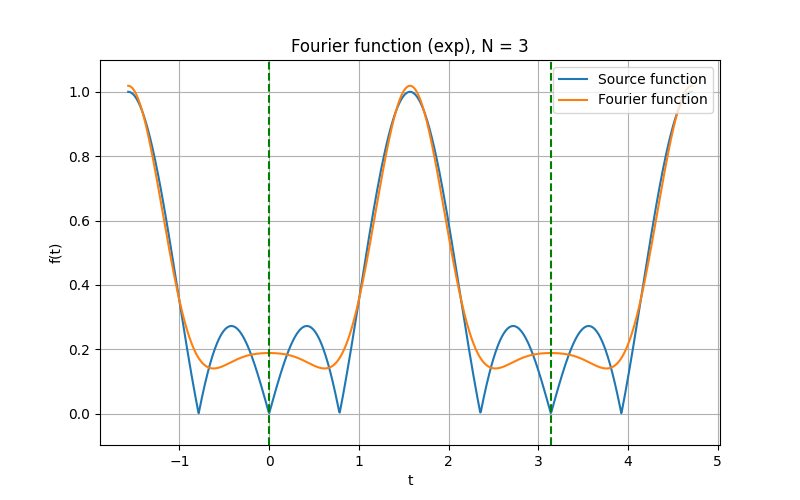
\includegraphics[width=0.49\textwidth]{media/plots/func_3_exp_N_3.png}
    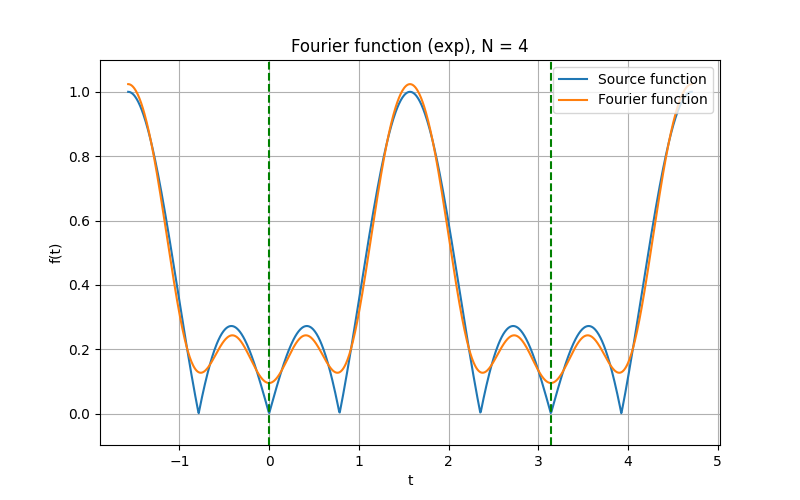
\includegraphics[width=0.49\textwidth]{media/plots/func_3_exp_N_4.png}
    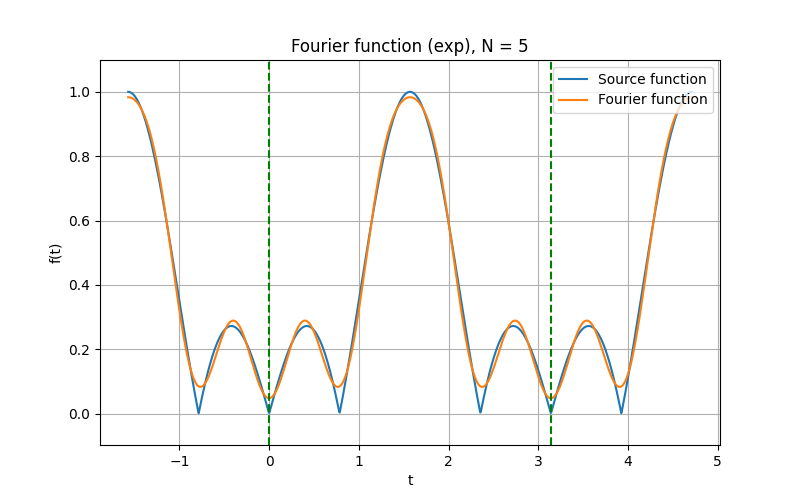
\includegraphics[width=0.49\textwidth]{media/plots/func_3_exp_N_5.png}
    \caption{График частичных сумм ряда Фурье для функции $f_3(t)$}
    \label{fig:func_3_plot_exp}
\end{figure}


Видим, что при увеличении $N$ график частичной суммы ряда Фурье приближается к исходной функции, но, в отличие от четной функции, не становится неотличимым от исходной функции при $N = 5$.

\FloatBarrier
\subsubsection{Проверка равенства Парсеваля}

Проверим равенство Парсеваля для функции $f_3(t)$:

Для этого воспользуемся функцией \texttt{perseval\_check} (см. листинг~\ref{lst:perseval_check}).
Мною была рассмотрена сумма трехсот коэффициентов. Этого оказалось достаточно для равенства квадрата нормы и суммы до 6 знака. 

\begin{table}[ht!]
    \centering
    \begin{tabular}{|c|c|c|}
        \hline
        $||f_3||^2$ & $2\pi \sum\limits_{n = -\infty}^{300} |c_n|^2$ & $\pi \left(\frac{a_0^2}{2} + \sum\limits_{n = 1}^{300} (a_n^2 + b_n^2)\right)$\\
        \hline
        1.57080 & 1.57080 & 1.57080 \\
        \hline
    \end{tabular}
    \caption{Проверка равенства Персеваля для функции $f_3(t)$}
    \label{tab:func_3_pers}
\end{table}
\FloatBarrier

\subsection{Ни нечетная, ни четная функция}

Рассмотрим периодическую функцию с периодом $T = 2\pi$:

\begin{equation}
    f_4(t) = \sin(t)^3 - \cos(t)
\end{equation}

График этой функции приведен на рис.~\ref{fig:func_4}.

\begin{figure}[ht!]
    \centering
    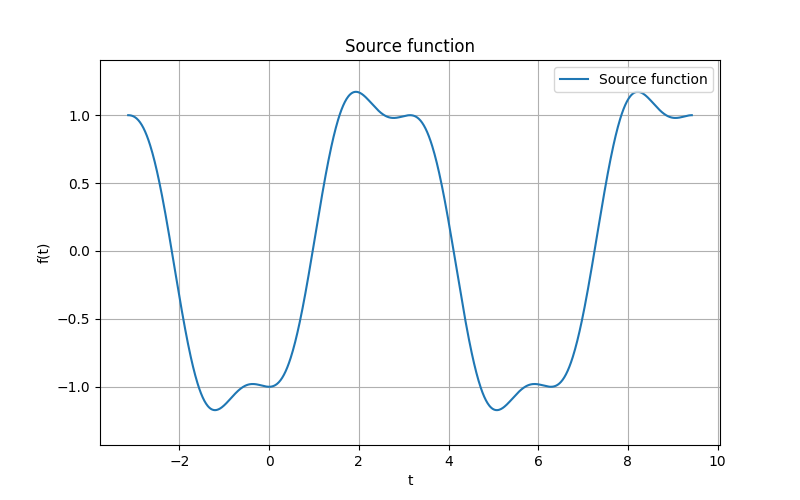
\includegraphics[width=\textwidth]{media/plots/func_4.png}
    \caption{График функции $f_4(t)$}
    \label{fig:func_4}
\end{figure}

\subsubsection{Вычисление коэффициентов Фурье}
Найдем коэффициенты ряда Фурье для этой функции:

\begin{equation}
    a_n = \frac{1}{\pi}\int\limits_{-\pi}^{\pi} (\sin(t)^3 - \cos(t)) \cos(n t) dt 
\end{equation}

\begin{equation}
    b_n = \frac{1}{\pi}\int\limits_{-\pi}^{\pi} (\sin(t)^3 - \cos(t)) \cos(n t) dt 
\end{equation}

\begin{equation}
    c_n = \frac{1}{2\pi}\int\limits_{-\pi}^{\pi} (\sin(t)^3 - \cos(t)) e^{-int} dt
\end{equation}

\subsubsection{Вычисление коэффициентов Фурье с помощью программы}

\begin{lstlisting}[style=python_white, caption=Вычисление коэффициентов Фурье, label=lst:func_4]
func = np.vectorize(lambda x: np.sin(x) ** 3 - np.cos(x))
a, b = fourier(func, 0, 2 * np.pi, 3)
print_fourier_coefficients(a, b)
c = fourier_exp(func, 0, 2 * np.pi, 3)
print_fourier_exp_coefficients(c)
\end{lstlisting}

В результате выполнения программы (\ref{lst:func_4}) получим следующие значения (см. таблицу~\ref{tab:func_4}~и~\ref{tab:func_4_exp}).

% table with coefficients
\begin{table}[ht!]
    \centering
    \begin{tabular}{|c|c|c|}
        \hline
        $n$ & $a_n$ & $b_n$ \\
        \hline
        0 & -0.00020 & 0.00000\\
        1 & -1.00020 & 0.75000\\
        2 & -0.00020 & 0.00000\\
        3 & -0.00020 & -0.25000\\
        \hline
    \end{tabular}
    \caption{Коэффициенты Фурье для функции $f_4(t)$}
    \label{tab:func_4}
\end{table}

\begin{table}[ht!]
    \centering
    \begin{tabular}{|c|c|}
        \hline
        $n$ & $c_n$ \\
        \hline
        -3 & -0.00010-0.12500i \\
        -2 & -0.00010-0.00000i \\
        -1 & -0.50010+0.37500i \\
        0 & -0.00010+0.00000i \\
        1 & -0.50010-0.37500i \\
        2 & -0.00010+0.00000i \\
        3 & -0.00010+0.12500i \\
        \hline
    \end{tabular}
    \caption{Коэффициенты Фурье для функции $f_4(t)$ (комплексный случай)}
    \label{tab:func_4_exp}
\end{table}

\subsubsection{Построение графиков частичных сумм ряда Фурье}
В качество значений $N$ выберем $N = 1, 2, 3, 4, 5$. Для каждого значения $N$ вычислим частичную сумму ряда Фурье и построим график (см. рис.~\ref{fig:func_4_plot}~и~\ref{fig:func_4_plot_exp}).

\begin{lstlisting}[style=python_white, caption=Построение графиков частичных сумм ряда Фурье, label=lst:func_1_plot]
func = np.vectorize(lambda x: np.sin(x) ** 3 - np.cos(x))
calc_and_plot(func, 0, 2 * np.pi, [1, 2, 3, 4, 5], './media/plots/func_4')
calc_and_plot_exp(func, 0, 2 * np.pi, [1, 2, 3, 4, 5], './media/plots/func_4_exp')
\end{lstlisting}

% plot with partial sums
\begin{figure}[ht!]
    \centering
    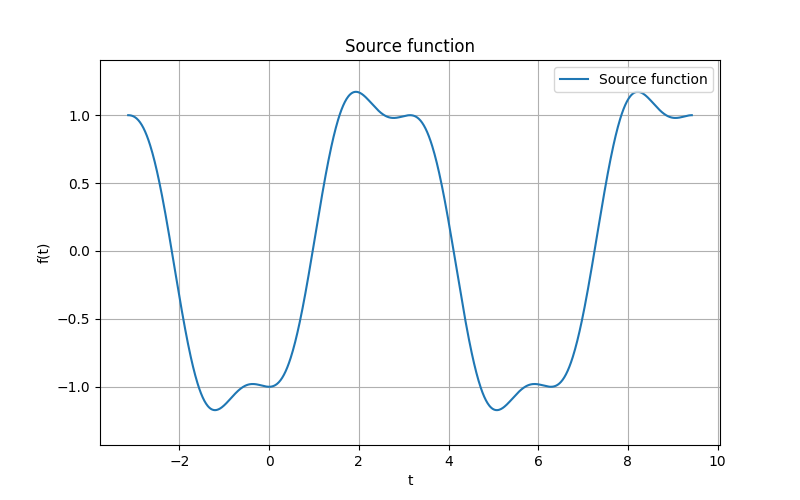
\includegraphics[width=0.49\textwidth]{media/plots/func_4.png}
    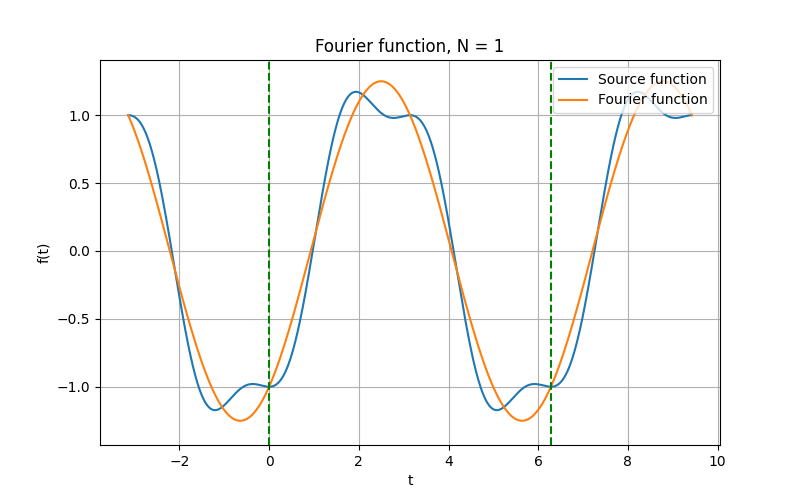
\includegraphics[width=0.49\textwidth]{media/plots/func_4_N_1.png}
    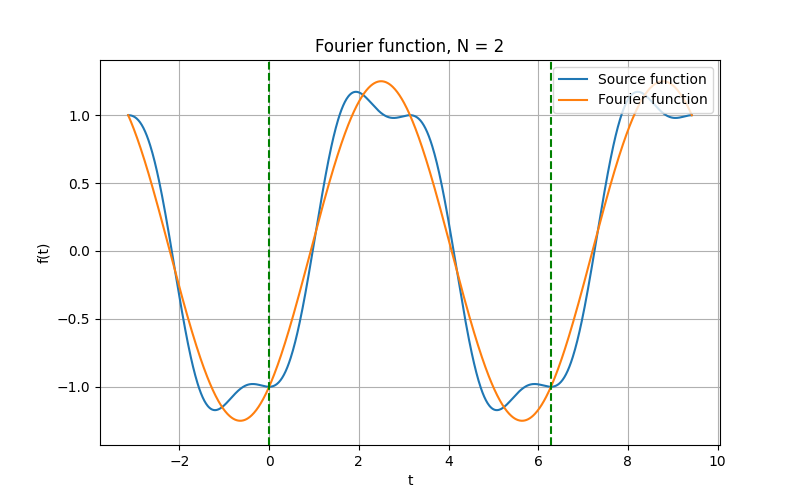
\includegraphics[width=0.49\textwidth]{media/plots/func_4_N_2.png}
    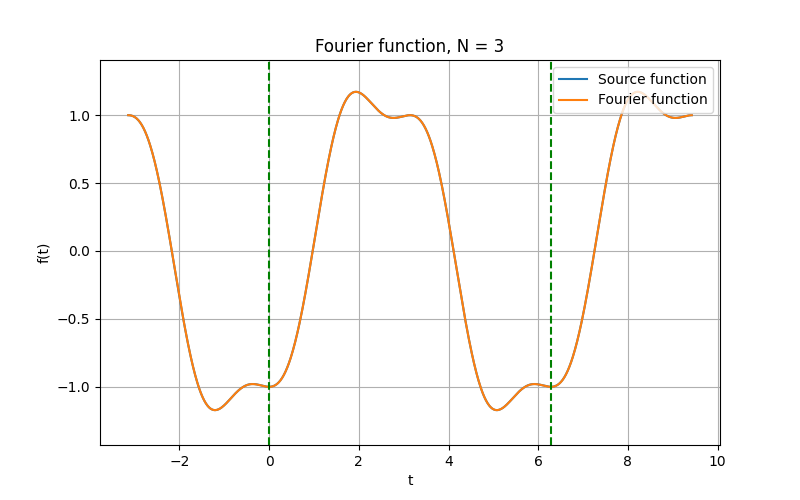
\includegraphics[width=0.49\textwidth]{media/plots/func_4_N_3.png}
    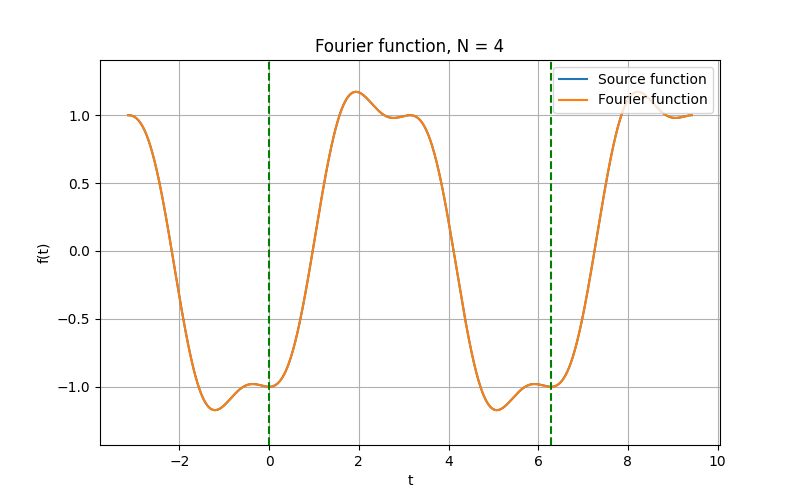
\includegraphics[width=0.49\textwidth]{media/plots/func_4_N_4.png}
    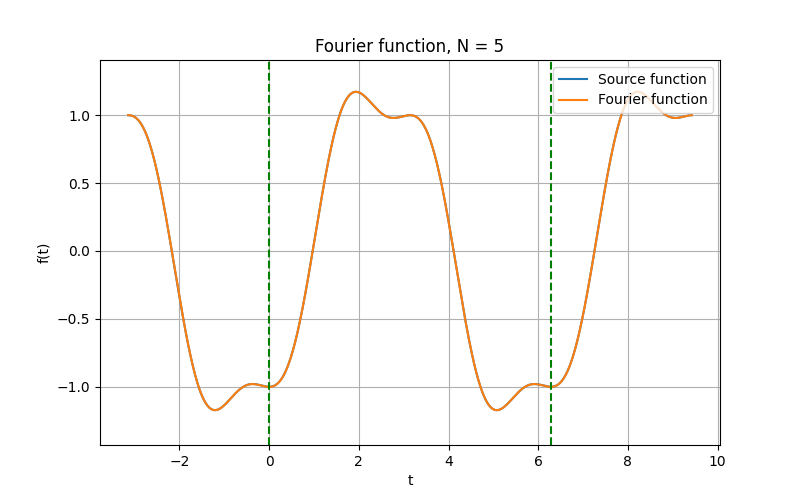
\includegraphics[width=0.49\textwidth]{media/plots/func_4_N_5.png}
    \caption{График частичных сумм ряда Фурье для функции $f_4(t)$}
    \label{fig:func_4_plot}
\end{figure}

\begin{figure}[ht!]
    \centering
    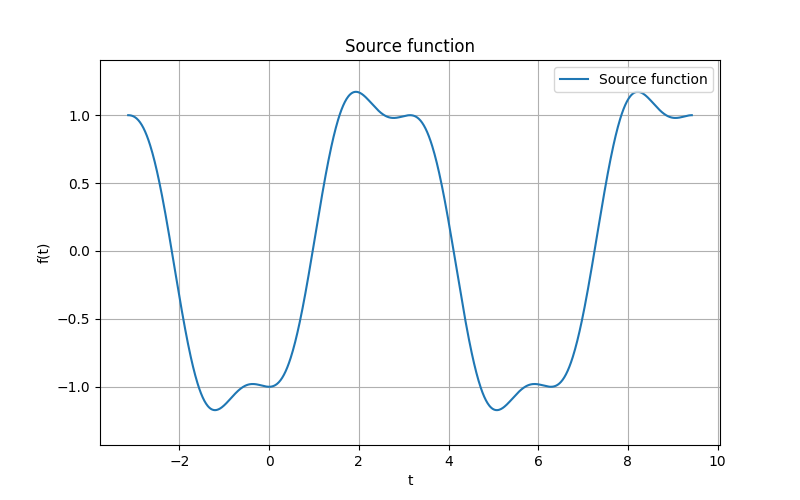
\includegraphics[width=0.49\textwidth]{media/plots/func_4_exp.png}
    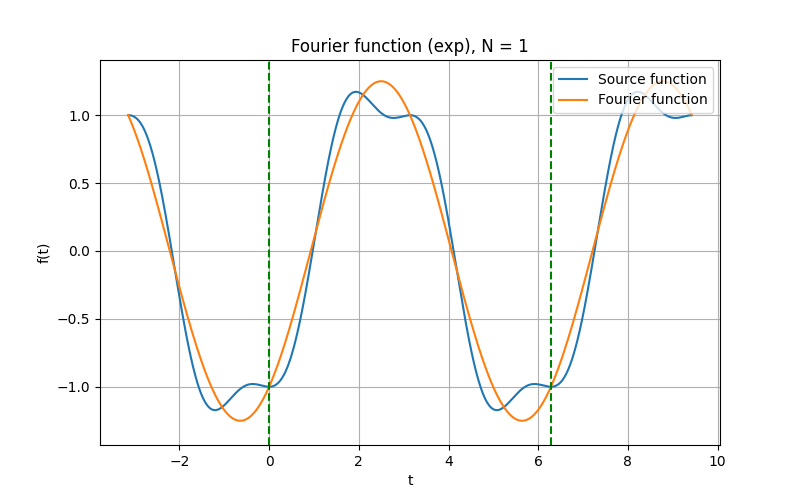
\includegraphics[width=0.49\textwidth]{media/plots/func_4_exp_N_1.png}
    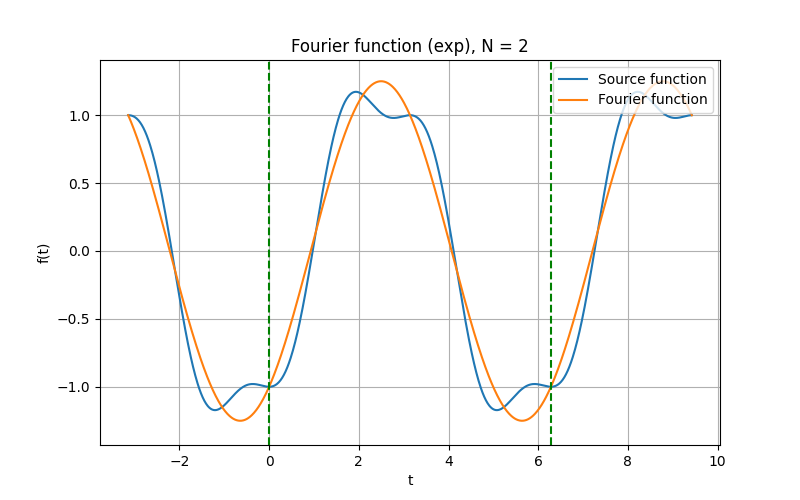
\includegraphics[width=0.49\textwidth]{media/plots/func_4_exp_N_2.png}
    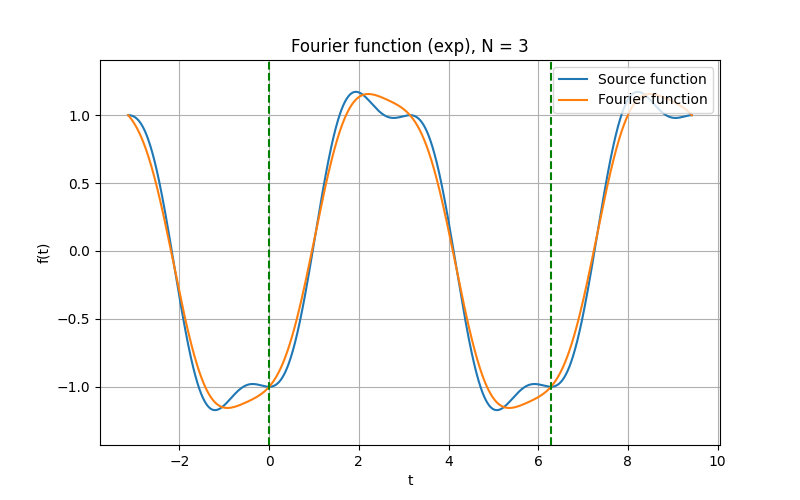
\includegraphics[width=0.49\textwidth]{media/plots/func_4_exp_N_3.png}
    \includegraphics[width=0.49\textwidth]{media/plots/func_4_exp_N_4.png}
    \includegraphics[width=0.49\textwidth]{media/plots/func_4_exp_N_5.png}
    \caption{График частичных сумм ряда Фурье для функции $f_4(t)$}
    \label{fig:func_4_plot_exp}
\end{figure}

Видим, что при увеличении $N$ график частичной суммы ряда Фурье приближается к исходной функции, и уже при $N = 3$ график частичной суммы ряда Фурье неотличим от исходной функции.

\FloatBarrier

\subsection{Анализ результатов}
Как и ожидалось, с увеличением количества коэффициентов график частичной суммы ряда Фурье (см. формулы~\ref{eq:fourier}~и~\ref{eq:fourier_exp}) 
все точнее приближают исходную функцию. При этом, у функции, которая терпит разрывы первого рода в точках, наблюдаются \textit{выбросы} в этих точках. 
Это связано с тем, что частичная сумма ряда Фурье не сходится к функции равномерно, а сходится по норме. 

Во всех случаях удалось убедиться в выполнении равенства Парсеваля. Квадрат нормы функции равен сумме квадратов модулей коэффициентов ряда Фурье с точностью, как минимум, до 3 знаков после запятой.

Графики частичных сумм ряда Фурье для вещественного и комплексного случая не отличаются. 
\FloatBarrier

\section{Комплексная функция}
\subsection{Комплексный квадрат}
Рассмотрим комплексную функцию  $f_5(t)$:

\begin{equation}
    Re f_5(t) = \begin{cases}
        3, & t \in [-\frac{1}{2}, \frac{1}{2})\\[0.75pt]
        6 - 6t, & t \in [\frac{1}{2}, \frac{3}{2})\\[0.75pt]
        -3, & t \in [\frac{3}{2}, \frac{5}{2})\\[0.75pt]
        -18 + 6t, & t \in [\frac{5}{2}, \frac{7}{2})\\[0.75pt]
    \end{cases} 
    ~~~~~
    Im f_5(t) = \begin{cases}
        6t, & t \in [-\frac{1}{2}, \frac{1}{2})\\[0.75pt]
        3, & t \in [\frac{1}{2}, \frac{3}{2})\\[0.75pt]
        12 - 6t, & t \in [\frac{3}{2}, \frac{5}{2})\\[0.75pt]
        -3, & t \in [\frac{5}{2}, \frac{7}{2})\\[0.75pt]
    \end{cases}
\label{eq:complex_func}
\end{equation}

График этой функции представлен на рисунке~\ref{fig:complex_func}.

\begin{figure}[ht!]
    \centering
    \includegraphics[width=\textwidth]{./media/plots/func_5.png}
    \caption{График комплексной функции $f_5(t)$}
    \label{fig:complex_func}
\end{figure}

\subsubsection{Вычисление коэффициентов Фурье}
Найдем коэффициенты ряда Фурье для этой функции в соответствии с формулой~\ref{eq:fourier_coefficients_exp}.

\begin{multline}
    c_n = \frac{1}{4}\int\limits_{-0.5}^{3.5} f_5(t) e^{-i \frac{\pi nt}{2}} dt = \frac{1}{4} ( \int\limits_{-0.5}^{0.5} (3 + 6ti)e^{-i \frac{\pi nt}{2}} dt + \int\limits_{0.5}^{1.5} (6 - 6t + 3i)e^{-i \frac{\pi nt}{2}} dt \\
    + \int\limits_{1.5}^{2.5}(-3 + (12 - 6t)i) e^{-i \frac{\pi nt}{2}} dt + \int\limits_{2.5}^{3.5}(-18 + 6t - 3i) e^{-i \frac{\pi nt}{2}} dt )
\end{multline}

\subsubsection{Вычисление коэффициентов Фурье с помощью программы}

\begin{lstlisting}[style=python_white, caption=Вычисление коэффициентов Фурье, label=lst:func_5]
R = 3
T = 4

def func(t):
    real = -1
    if -T/8 <= t < T/8:
        real = R
    if T/8 <= t < 3 * T / 8:
        real = 2 * R - 8 * R * t / T 
    if 3 * T / 8 <= t < 5 * T / 8:
        real = -R
    if 5 * T / 8 <= t <= 7 * T / 8:
        real = -6 * R + 8 * R * t / T

    imag = -1
    if -T/8 <= t < T/8:
        imag = 8 * R * t / T
    if T/8 <= t < 3 * T / 8:
        imag = R
    if 3 * T / 8 <= t < 5 * T / 8:
        imag = 4 * R - 8 * R * t / T
    if 5 * T / 8 <= t <= 7 * T / 8:
        imag = -R

    return real + 1j * imag

func = np.vectorize(func)
c = fourier_exp(func, -T/8, T, 3)
print_fourier_exp_coefficients(c)
\end{lstlisting}

В результате выполнения программы (\ref{lst:func_5}) получим следующие значения (см. таблицу~\ref{tab:func_5_exp}).

\begin{table}[h!]
    \centering
    \begin{tabular}{|c|c|}
        \hline
        $n$ & $c_n$ \\
        \hline
        -3 & -0.38253+0.00000i \\
        -2 & -0.00030-0.00030i \\
        -1 & -0.00000-0.00042i \\
        0 & 0.00030-0.00030i \\
        1 & 3.43938+0.00000i \\
        2 & 0.00030+0.00030i \\
        3 & -0.00000+0.00042i \\
        \hline
    \end{tabular}
    \caption{Коэффициенты Фурье для функции $f_5(t)$ }
    \label{tab:func_5_exp}
\end{table}

\subsubsection{Построение графиков частичных сумм ряда Фурье}
В качество значений $N$ выберем $N = 1, 2, 3, 5, 10$. Для каждого значения $N$ вычислим частичную сумму ряда Фурье и построим график (см. рис.~\ref{fig:func_5_plot}).

\begin{lstlisting}[style=python_white, caption=Построение графиков частичных сумм ряда Фурье, label=lst:func_1_plot]
    calc_and_plot_parametric(func, -T/8, T, [1, 2, 3, 5, 10], './media/plots/func_5')
\end{lstlisting}

% plot with partial sums
\begin{figure}[ht!]
    \centering
    \includegraphics[width=0.49\textwidth]{media/plots/func_5.png}
    \includegraphics[width=0.49\textwidth]{media/plots/func_5_N_1.png}
    \includegraphics[width=0.49\textwidth]{media/plots/func_5_N_2.png}
    \includegraphics[width=0.49\textwidth]{media/plots/func_5_N_3.png}
    \includegraphics[width=0.49\textwidth]{media/plots/func_5_N_5.png}
    \includegraphics[width=0.49\textwidth]{media/plots/func_5_N_10.png}
    \caption{Параметрический график частичных сумм ряда Фурье для функции $f_5(t)$}
    \label{fig:func_5_plot}
\end{figure}

Видим, что как и в случае вещественных функций, при увеличении значения $N$ график частичной суммы ряда Фурье все точнее приближает исходную функцию. 
При значениях $N = 1, 2$ график частичной суммы ряда Фурье представляет из себя эллипс, при $N = 3$ -- уже похож на исходную функцию.
При значениях $N = 10$ график частичной суммы ряда Фурье довольно точно повторяет исходную функцию.

\subsection{Графики вещественной и комплексной части отдельно}

Рассмотрим графики $Re~f_5(t)$ и $Im~f_5(t)$ (см. рис.~\ref{fig:func_5_re_im}) и графики $Re~G_n(t)$ и $Im~G_n(t)$  для функции $f_5(t)$ (см. рис.~\ref{fig:func_5_fourier_re_im_N_1}~-~\ref{fig:func_5_fourier_re_im_N_10}).

\begin{figure}[ht!]
    \centering
    \includegraphics[width=0.49\textwidth]{media/plots/func_5_real.png}
    \includegraphics[width=0.49\textwidth]{media/plots/func_5_imag.png}
    \caption{График  $f_5(t)$ (действительная и мнимая часть)}
    \label{fig:func_5_re_im}
\end{figure}


\begin{figure}[ht!]
    \centering
    \includegraphics[width=0.49\textwidth]{media/plots/func_5_real_N_1.png}
    \includegraphics[width=0.49\textwidth]{media/plots/func_5_imag_N_1.png}
    \caption{График частичных сумм ряда Фурье для функции $f_5(t)$ ($N = 1$) (действительная и мнимая часть)}
    \label{fig:func_5_fourier_re_im_N_1}
\end{figure}

\begin{figure}[ht!]
    \centering
    \includegraphics[width=0.49\textwidth]{media/plots/func_5_real_N_2.png}
    \includegraphics[width=0.49\textwidth]{media/plots/func_5_imag_N_2.png}
    \caption{График частичных сумм ряда Фурье для функции $f_5(t)$ ($N = 2$) (действительная и мнимая часть)}
    \label{fig:func_5_fourier_re_im_N_2}
\end{figure}

\begin{figure}[ht!]
    \centering
    \includegraphics[width=0.49\textwidth]{media/plots/func_5_real_N_3.png}
    \includegraphics[width=0.49\textwidth]{media/plots/func_5_imag_N_3.png}
    \caption{График частичных сумм ряда Фурье для функции $f_5(t)$ ($N = 3$) (действительная и мнимая часть)}
    \label{fig:func_5_fourier_re_im_N_3}
\end{figure}


\begin{figure}[ht!]
    \centering
    \includegraphics[width=0.49\textwidth]{media/plots/func_5_real_N_5.png}
    \includegraphics[width=0.49\textwidth]{media/plots/func_5_imag_N_5.png}
    \caption{График частичных сумм ряда Фурье для функции $f_5(t)$ ($N = 5$) (действительная и мнимая часть)}
    \label{fig:func_5_fourier_re_im_N_5}
\end{figure}

\begin{figure}[ht!]
    \centering
    \includegraphics[width=0.49\textwidth]{media/plots/func_5_real_N_10.png}
    \includegraphics[width=0.49\textwidth]{media/plots/func_5_imag_N_10.png}
    \caption{График частичных сумм ряда Фурье для функции $f_5(t)$ ($N = 10$) (действительная и мнимая часть)}
    \label{fig:func_5_fourier_re_im_N_10}
\end{figure}

Тут так же заметно, что с увеличением значения $N$ график частичной суммы ряда Фурье все точнее приближает исходную функцию на выбранном промежутке. 

\clearpage

\section{Дополнительное задание}
\subsection{Разложение рисунка}
По аналогии с разложением комплексной параметрической функции, можно найти разложение в ряд Фурье для функции, график которой представляет из себя интересующий нас рисунок. 

Нам подойдет рисунок в векторном формате, который состоит из одной замкнутой линии. Она не должна иметь толщины. В редакторе CoralDraw для этого существует параметр \textit{сверхтонкий абрис}. 

\begin{figure}[ht!]
    \centering
    \includegraphics[width=0.5\textwidth]{./media/cat.jpg}
    \caption{Рисунок, который будет раскладывать}
    \label{fig:cat}
\end{figure}

Возьмем рисунок с котиком. Для того, чтобы \textit{достать} параметрический график из svg файла можно использовать библиотеку \texttt{svg.path} и ее функцию \texttt{parse\_path}. 

\begin{lstlisting}[style=python_white, caption={Получение параметрической функции рисунка}, label=lst:parametric_function]
path = svg.path.parse_path(spline)
path_func = np.vectorize(lambda t: path.point(t) * scale)
\end{lstlisting}

В результате работы кода (см. листинг~\ref{lst:parametric_function}) получаем параметрическую функцию $path\_func(t)$, где $t \in [0, 1]$, 
которая будет возвращать точку на комплексной плоскости. 

Теперь данную функцию можно разложить в ряд Фурье на отрезке $[0, 1]$ с помощью функции \texttt{fourier\_exp} (см. листинг~\ref{lst:fourier_cat}). 
В результате работы этой функции получим набор коэффициентов $c_n$, которые являются коэффициентами искомого разложения рисунка. 

Для проверки полученного результата можно построить \textit{графики} полученных функций (количество коэффициентов $N=20$) (см рис. \ref{fig:cat_plot}). 
Видим, что оба графика крайне похожи друг на друга. Это значит, что разложение Фурье корректно применилось для нашего рисунка. 

\begin{figure}[ht!]
    \centering
    \includegraphics[width=0.49\textwidth]{./media/cat_func.png}
    \includegraphics[width=0.49\textwidth]{./media/cat_fourier.png}
    \caption[]{Исходный рисунок и рисунок после разложения Фурье ($N = 20$)}
    \label{fig:cat_plot}
\end{figure}

\subsection{Вращаем векторы}
Теперь разберемся с тем, как можно представить полученные коэффициенты разложения с виде движущихся с целой частотой относительно друг друга векторов. 

Из разложения (см. формулу \ref{eq:fourier_exp}) мы имеем слагаемые вида:
\begin{equation}
    c_i\cdot e^{i\omega_it}
    \notag
\end{equation}
Каждый из коэффициентов $c_i$ имеет комплексное значение, при этом $i$ определяет частоту вращения вектора (об/ceк, если $i < 0$, то вращение в другую сторону).

Для определения радиуса круга с номером (и частотой вращения) $i$ можно воспользоваться следующей формулой: 
\begin{equation}
    r = \sqrt{Re(c_i)^2 + Im(c_i)^2}
\end{equation}
Это будет радиус окружности, внутри которой вращается вектор. 

Начальное положение вектора будем задавать как часть дуги (от 0 до 1), на которую должен \textit{указывать} вектор. Обозначим это значение $\phi$
Найти его можно следующим образом: 
\begin{equation}
    \phi = \begin{cases}
        \frac{atan2(-Im(c_i),~Re(c_i))}{2\pi} & atan2(Im(c_i), Re(c_i)) > 0\\
        \frac{atan2(-Im(c_i),~Re(c_i)) + 2\pi}{2\pi} & atan2(Im(c_i), Re(c_i)) <= 0
    \end{cases}
\end{equation}
После мнимой части стоит минус для того, чтобы рисунок не был перевернутым. 

Теперь, когда у нас есть все нужные значения (частоты вращения векторов, длины векторов, начальные положения), мы можем перейти к отрисовке. 

\subsection{Отрисовка графики}

Основной единицей в программе являются объект класса \texttt{RotatingCircle} (см. листинг~\ref{lst:rotating_circle}), который наследован от класса \texttt{Circle} -- вращающаяся окружность. 
В нем добавлены поля, хранящие окружность, по орбите которой она вращается, частота вращения и позиции \textit{точки} на этой окружности. 

Кроме того, добавлены классы \texttt{VectorInCircle} и \texttt{DotOnCircle}, наследованные от классов 
\texttt{Arrow} и \texttt{Dot} соответственно. Они нужны лишь для визуализации соответствующих элементов. 

Все \textit{действие} основано на обновлении точек на окружностях, и, соответственно, центов окружностей, которые привязных к этим точках.

Функция \texttt{rotating\_circle\_updater} изменяет положение точки на окружности, \texttt{dot\_on\_circle\_updater} -- перемещает точку по окружности, \texttt{vector\_in\_circle\_updater} -- перемещает начало вектора в центр окружности, в которой он расположен и конец вектора к точке на этой же окружности. 

Таким образом, изменение положения центра окружности и положения точки на ней ведет к изменений положения всех элементов. 

В основном методе рассчитываются коэффициенты $c_i$ и создаются \textit{вложенные} окружности (родителем каждой следующей окружности является предыдущая), центр которых привязывается к точке на родительской окружности. 
Таким образом создается зависимость положения дочерних окружностей от родительских. 

В результате получаем анимацию с отрисовкой исходного рисунка (\href{https://drive.google.com/file/d/1bMOGz81cHuQbmYTLcZKFB8C2WC-LNEim/view?usp=share_link}{ссылка}):  

Так же можно посмотреть на анимации при различных значениях $N$ (\href{https://drive.google.com/drive/folders/1dmXw8v6x5eByshXMqzxIWHGvhgOteTDo?usp=share_link}{ссылка}). 

Исходный код находится в приложении \ref{appendix:appendixB}. 

\begin{figure}[ht!]
    \centering
    \includegraphics[width=0.6\textwidth]{./media/cat_animation.png}
    \label{fig:cat_animation}
    \caption{Стоп-кадр из анимации}
\end{figure}
Полученный рисунок полностью совпадает с тем, что был получен из частичной сумму ряда Фурье (см. рис.~\ref{fig:cat_plot}).